\documentclass[UTF8,openany]{ctexbook}

\usepackage{geometry}
\geometry{a4paper,left=2.5cm,right=2.5cm,top=2.5cm,bottom=2.5cm}
\usepackage[hidelinks]{hyperref}
\usepackage{graphicx}
\usepackage{float}
\usepackage{amsmath}
\usepackage{amssymb}
\usepackage{booktabs}
\usepackage{array}
\usepackage{longtable}
\usepackage{xcolor}
\usepackage{listings}
\usepackage{fancyhdr}
\graphicspath{{figures/}}
\setCJKfamilyfont{xingkai}{STXingkai}

\pagestyle{fancy}
\fancyhf{}
\fancyfoot[C]{\thepage}
\renewcommand{\headrulewidth}{0pt}
\renewcommand{\footrulewidth}{0pt}
\fancypagestyle{plain}{%
    \fancyhf{}
    \fancyfoot[C]{\thepage}
    \renewcommand{\headrulewidth}{0pt}
    \renewcommand{\footrulewidth}{0pt}
}

\lstset{
    basicstyle=\ttfamily\small,
    breaklines=true,
    frame=single,
    columns=fullflexible,
    backgroundcolor=\color{gray!5},
    keywordstyle=\color{blue!60!black},
    commentstyle=\color{green!40!black}
}

\newcommand{\coverfield}[2]{%
    #1 & \underline{\makebox[9.2cm][c]{#2}}\\[0.75cm]
}

\newcommand{\makecoursecover}{%
\begin{titlepage}
    \thispagestyle{empty}
    \begin{center}
        \vspace*{1.6cm}
        {\CJKfamily{xingkai}\zihao{2} 武汉大学国家网络安全学院\par}

        \vspace{2.2cm}
        {\songti\zihao{1} 公钥密码学实验\par}
        \vspace{0.35cm}
        {\songti\zihao{1} 期末实验报告\par}
    \end{center}

    \vspace{2.4cm}
    \begin{center}
        {\songti\zihao{4}
        \begin{tabular}{rl}
            \coverfield{题\hspace{1.2em}目：}{基于 LSSS 矩阵的属性基加密方案}
            \coverfield{专业(班)：}{密码科学与技术试验班}
            \coverfield{学\hspace{1.2em}号：}{2024302182033}
            \coverfield{姓\hspace{1.2em}名：}{黄德林}
            \coverfield{课程名称：}{公钥密码学实验}
            \coverfield{任课教师：}{宁建廷}
        \end{tabular}
        }
    \end{center}
    \vfill
\end{titlepage}
}

\begin{document}

\pagenumbering{gobble}
\makecoursecover
\tableofcontents
\clearpage
\pagenumbering{arabic}

\chapter{实验目的与任务说明}

\section{实验背景}

属性基加密（Attribute-Based Encryption, ABE）是一类将访问控制机制嵌入密码算法的公钥加密技术。与传统公钥加密“为某一个具体接收者加密”不同，ABE 允许加密方围绕属性集合或访问策略表达授权条件。例如，一个文件可以被加密给“部门为研发且安全级别不低于三级”的所有用户，而不是某一个固定身份的用户。这样的机制适合云存储、数据共享、组织权限管理和细粒度访问控制等场景。

本实验选择密文策略属性基加密（Ciphertext-Policy ABE, CP-ABE）作为实现对象。在 CP-ABE 中，密文携带访问策略，用户私钥携带属性集合。用户能否解密不由单一身份决定，而由其属性集合是否满足密文中的策略决定。本项目进一步选取线性秘密共享方案（Linear Secret Sharing Scheme, LSSS）作为访问策略的内部表示方法，将访问控制树转换为矩阵，并在解密端通过线性方程求解完成秘密重构。

因此，本实验并不是单纯实现一个“能加密、能解密”的命令行程序，而是围绕三个问题展开：第一，如何把直观的访问控制树转换为可计算的 LSSS 矩阵；第二，如何在 CP-ABE 的加密和解密过程中使用这些矩阵行；第三，如何通过实验说明满足策略和不满足策略时的行为差异。后续章节均围绕这三个问题展开，避免把算法、代码和实验结果割裂成互不相干的部分。

本报告的写作和实现均以 \verb|References_Article| 目录中的课程文件和论文为主要依据。课程期末文件将本题表述为“基于 LSSS 矩阵的属性基加密方案（使用访问控制树构建 LSSS 矩阵）”；实验三课件~[1]围绕 Waters 2011 方案~[3]与 FABEO 方案~[5]的实现与测试展开，给出了访问矩阵、属性映射、加密向量和解密重构常数等核心符号。因此，本项目把课程要求中的“访问控制树构建 LSSS 矩阵”作为实现主线，以实验三课件~[1]中的 Waters 2011 伪代码作为 CP-ABE 算法结构参照，并结合 Bethencourt、Sahai 和 Waters 提出的 CP-ABE 方案~[2]、Waters 的 LSSS-CP-ABE 构造~[3]以及 Liu、Cao 和 Wong 关于阈值访问树生成 LSSS 矩阵的研究~[4]补充理论依据。

\section{实验任务}

期末大作业要求在若干题目中任选一题完成完整实验报告和软件系统源码。本项目对应的题目是“基于 LSSS 矩阵的属性基加密方案（使用访问控制树构建 LSSS 矩阵）”。围绕这一要求，项目完成以下任务：

\begin{enumerate}
    \item 设计一种 JSON 格式的访问控制树表示方法，支持叶子属性、AND、OR 和一般阈值门。
    \item 实现从访问控制树到 LSSS 矩阵 $(M,\rho)$ 的转换算法。
    \item 实现 CP-ABE 的四个核心流程：Setup、KeyGen、Encrypt 和 Decrypt。
    \item 使用指数抽象模型验证 CP-ABE 的代数正确性。
    \item 在同一 \verb|Project| 工程中接入 BLS12-381 真实双线性配对库，验证同一访问结构在真实群元素上的可运行性。
    \item 使用 AES-CBC 与 HMAC-SHA256 完成明文载荷的对称加密和完整性校验。
    \item 提供命令行脚本和烟雾测试，使实验可以在 Windows PowerShell 环境中复现。
    \item 编写配套实验报告，解释理论基础、系统设计、实现细节和实验结果。
\end{enumerate}

上述任务中，最关键的是第二项、第三项和第五项。访问控制树到 LSSS 矩阵的转换决定了系统能否支持 AND、OR 和一般阈值门；Setup、KeyGen、Encrypt 和 Decrypt 四个流程则决定了矩阵结果能否真正参与属性基加密；真实配对库接入则用于检查底层群运算从指数抽象切换到真实 $G_1/G_2/G_T$ 元素后，访问树、矩阵构造和重构求解是否仍能保持稳定。对称加密和命令行脚本属于工程支撑部分，它们保证实验对象不是停留在公式层面，而是能够处理真实文件、生成可检查的 JSON 结果，并通过测试脚本反复验证。

\section{项目组织}

本仓库的主要目录如下：

\begin{table}[H]
\centering
\caption{项目目录组织}
\begin{tabular}{>{\raggedright\arraybackslash}p{0.30\textwidth} >{\raggedright\arraybackslash}p{0.60\textwidth}}
\toprule
目录或文件 & 作用 \\
\midrule
\verb|README.md| & 项目总说明，概述系统功能、目录结构、运行入口和实现边界。\\
\verb|Project/bin/lsss-abe.ps1| & 命令行入口，负责解析 setup、keygen、encrypt、decrypt 四类命令。\\
\path{Project/src/LsssAbe/LsssAbe.psm1} & 核心 PowerShell 模块，包含数学工具、LSSS 构造、加解密算法和 JSON I/O。\\
\verb|Project/examples| & 示例策略文件和示例明文。\\
\verb|Project/tests/smoke.ps1| & 烟雾测试脚本，验证九个成功、失败和边界输入场景。\\
\path{Project/src/LsssAbe/pairing_backend.py} & 真实 BLS12-381 pairing 后端，负责执行真实群元素、配对、哈希到群和序列化相关运算。\\
\path{Project/tests/smoke_pairing.ps1} & 真实 pairing 路线烟雾测试脚本，验证 BLS12-381 后端下的核心成功、失败和边界场景。\\
\verb|Report/LaTeX| & 本实验报告的 LaTeX 工程，包含正文、图表、截图和最终 PDF。\\
\verb|References_Article| & 课程要求、实验课件和相关论文。\\
\bottomrule
\end{tabular}
\end{table}

这样的目录组织体现了本实验的两条主线：一条是可运行的算法实现，另一条是对算法原理、实现细节和实验现象的解释。\verb|Project| 目录集中保存命令行入口、核心模块、示例文件、指数抽象路线和真实 pairing 路线；两条路线共用访问树表示、LSSS 矩阵构造、重构求解和测试组织方式，差异主要体现在底层群元素表示和配对运算实现。\verb|Report/LaTeX| 目录用于把访问控制树、LSSS 矩阵、线性重构、真实群元素实现和程序输出对应起来。参考资料单独保存在 \verb|References_Article| 中，则便于在论述算法来源和实验要求时保持材料来源清晰。

\section{实验目标}

本实验的直接目标不是完成可部署密码库，而是清晰展示“访问策略如何被转换为线性代数问题”，以及 CP-ABE 中“满足策略才能解密”的机制如何在代码中落地。因此，本项目将目标划分为理论目标、算法目标、工程目标和验证目标。

\begin{table}[H]
\centering
\caption{实验目标分解}
\begin{tabular}{p{0.22\textwidth} p{0.68\textwidth}}
\toprule
目标类别 & 具体内容 \\
\midrule
理论目标 & 理解 CP-ABE、访问控制树、阈值门、LSSS 矩阵和线性重构之间的关系。\\
算法目标 & 实现树到矩阵转换、高斯消元求重构系数、CP-ABE 四个核心算法。\\
工程目标 & 构建可运行命令行系统，使用 JSON 存储密钥和密文，便于检查和复现。\\
验证目标 & 通过正例和反例验证满足策略与不满足策略时的解密行为。\\
\bottomrule
\end{tabular}
\end{table}

这些目标之间存在递进关系。理论目标回答“为什么 LSSS 能表达访问策略”；算法目标回答“如何从树构造矩阵并求解重构系数”；工程目标回答“如何把算法组织成可运行的软件”；验证目标回答“实验结果是否与策略语义一致”。如果只完成前三类目标而缺少验证，系统只能说明“代码写出来了”；如果缺少理论解释，测试通过也难以说明其与 LSSS-ABE 题目的对应关系。因此本报告在结构上同时保留公式推导、代码节选和实验结果。

\section{运行环境}

本项目选择 Windows PowerShell 作为主要命令行环境。基础实现使用 .NET 标准库提供的 \verb|System.Numerics.BigInteger|、\verb|System.Security.Cryptography| 等组件完成大整数运算、随机数生成、哈希、AES 和 HMAC，从而在不依赖第三方密码库的情况下展示访问结构、线性重构和解密抵消关系。为了进一步检查底层群运算真实化后的系统行为，真实 pairing 路线额外使用仓库根目录下的 conda 环境 \verb|env|，由 Python 后端调用 \verb|py-ecc| 的 BLS12-381 群运算和 \verb|pairing| 接口，并使用 \verb|pycryptodome| 完成 AES-CBC/HMAC 载荷处理。

实验环境由四部分组成：第一部分是 PowerShell 脚本运行环境，用于执行 Setup、KeyGen、Encrypt、Decrypt 和烟雾测试；第二部分是 .NET 标准库，用于提供大整数和基础密码组件；第三部分是 Python pairing 后端，用于真实 BLS12-381 群元素、哈希到群、配对和群元素序列化；第四部分是 LaTeX 编译环境，用于生成最终实验报告。各部分的作用如表 \ref{tab:runtime-env} 所示。

\begin{table}[H]
\centering
\caption{实验运行环境组成}
\label{tab:runtime-env}
\begin{tabular}{>{\raggedright\arraybackslash}p{0.26\textwidth} >{\raggedright\arraybackslash}p{0.60\textwidth}}
\toprule
环境组成 & 作用 \\
\midrule
Windows PowerShell & 作为命令行入口和脚本执行环境，负责运行四个核心算法命令和测试脚本。\\
.NET 大整数与密码学库 & 提供 \verb|BigInteger|、随机数生成、SHA-256、AES、HMAC 等基础能力。\\
Python \verb|py-ecc| 与 \verb|pycryptodome| & 为真实 pairing 路线提供 BLS12-381 的 $G_1/G_2/G_T/\mathbb{Z}_p$、真实配对、哈希到群和对称载荷加密能力。\\
JSON 文件格式 & 保存公共参数、主密钥、用户私钥、密文、访问树和 LSSS 矩阵，便于实验检查。\\
XeLaTeX & 编译中文实验报告，支持公式、表格、代码清单和截图排版。\\
\bottomrule
\end{tabular}
\end{table}

真实 pairing 路线所使用的 Python 环境如图 \ref{fig:pairing-dependencies} 所示。截图中记录了 Python 版本、\verb|py-ecc| 版本和 \verb|pycryptodome| 版本，其中 \verb|py-ecc| 提供 BLS12-381 曲线和 pairing 运算，\verb|pycryptodome| 提供对称加密与消息认证组件。该环境证据与表 \ref{tab:runtime-env} 中的 Python pairing 后端相对应。

\begin{figure}[H]
\centering
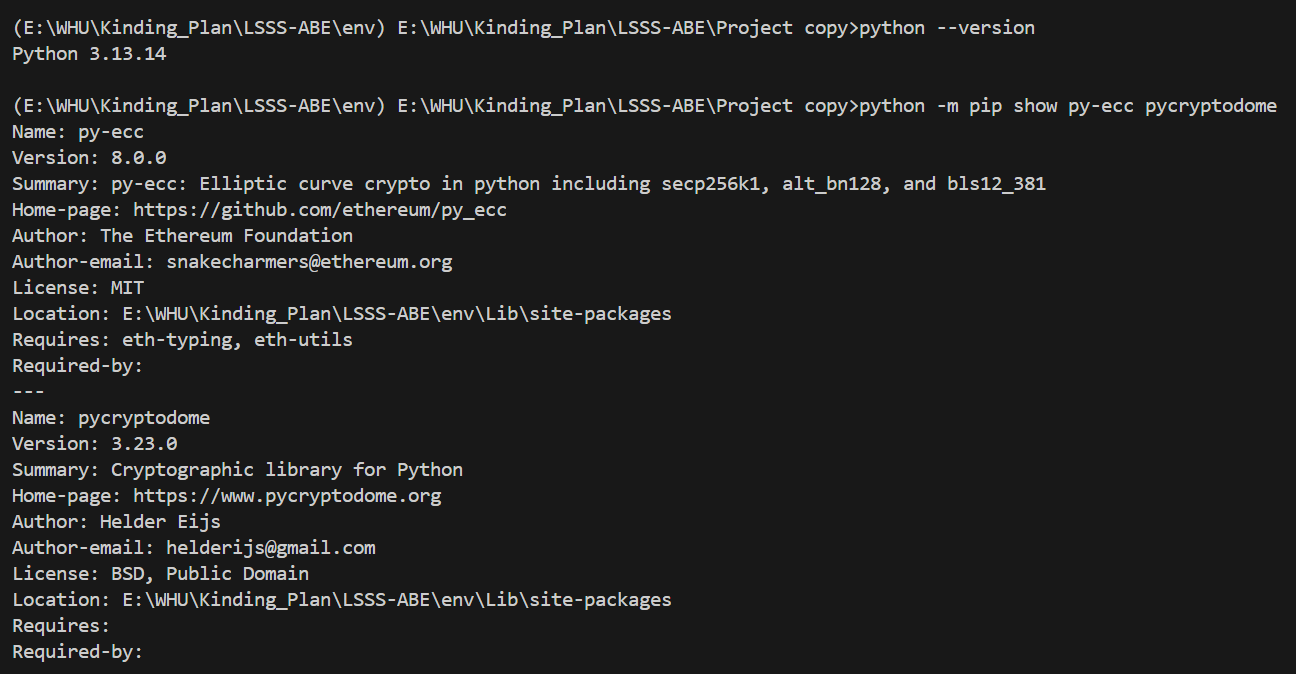
\includegraphics[width=0.95\textwidth]{pairing_dependencies.png}
\caption{真实 pairing 路线依赖环境截图}
\label{fig:pairing-dependencies}
\end{figure}

从实验复现角度看，PowerShell 脚本使四个算法阶段具有清晰边界。Setup 生成公共参数和主密钥，KeyGen 根据属性集合生成私钥，Encrypt 把访问树和明文转换为密文 JSON，Decrypt 根据用户私钥和密文恢复明文或给出拒绝信息。每个阶段都会留下可检查的文件结果，后续章节中的代码说明、JSON 字段和终端截图都与这些文件相对应。

烟雾测试命令如下：

\begin{lstlisting}[language=bash,caption={烟雾测试命令}]
powershell -NoProfile -ExecutionPolicy Bypass -File .\Project\tests\smoke.ps1
\end{lstlisting}

真实 pairing 路线的验证命令如下：

\begin{lstlisting}[language=bash,caption={真实 pairing 版烟雾测试命令}]
powershell -NoProfile -ExecutionPolicy Bypass -File .\Project\tests\smoke_pairing.ps1
\end{lstlisting}

命令中使用 \verb|-ExecutionPolicy Bypass|，是因为部分 Windows 机器默认禁止直接执行 \verb|.ps1| 脚本。该参数只影响当前进程，不会永久改变系统策略，因而适合本实验的临时复现环境。

\section{报告结构}

围绕“访问控制树构建 LSSS 矩阵并用于属性基加密”这一主题，本文依次展开理论基础、方案设计、系统实现、实验结果和总结展望。这样的安排遵循从抽象概念到程序实现、再到实验验证的顺序：先交代访问结构和 LSSS 的数学含义，再说明这些概念如何进入代码、文件和测试结果。

第二章说明属性基加密、CP-ABE、访问控制树、LSSS、双线性对和对称加密之间的关系。该章的作用是建立术语和公式基础，尤其说明为什么访问策略可以被转化为矩阵重构问题。第三章给出系统方案设计，重点描述访问树到 LSSS 的构造方法，以及 Setup、KeyGen、Encrypt、Decrypt 四个核心算法之间的数据流。第四章进入系统实现层面，说明 PowerShell 模块结构、数据结构、矩阵转换函数、重构求解和 CLI 入口。

第五章是实验过程与结果分析，围绕九个指数版测试场景和八类真实 pairing 版补充场景说明系统在满足策略、不满足策略、一般阈值门、重复属性、特殊属性名、密文篡改和非法策略输入下的行为。第六章对实验完成情况、实现边界和真实安全证明条件进行总结，并说明指数抽象模型与 BLS12-381 真实配对实现之间的关系。附录则保留完整命令清单、示例策略 JSON、核心伪代码和参考文献，作为正文分析的补充材料。

整体上，第一章提出任务和环境，第二章提供理论依据，第三章给出方案设计，第四章呈现实现细节，第五章提供实验证据，第六章收束结论和边界。各章之间形成“题目要求—理论模型—算法设计—代码实现—实验验证—结论分析”的链路。

\chapter{相关理论与关键概念}

\section{属性基加密的基本思想}

属性基加密（ABE）的核心思想是把“解密权利”从具体身份扩展为属性集合和访问结构之间的匹配关系。传统公钥加密要求加密者明确知道接收者的公钥；ABE 则允许系统使用“属性”和“访问策略”描述授权条件。需要区分的是，在 ABE 的一般定义中，访问策略不一定都放在密文中：CP-ABE 将访问策略嵌入密文、用户私钥携带属性集合；KP-ABE 则通常由密文携带属性集合、用户私钥携带访问策略。因此，更准确地说，ABE 的解密能力来自密文侧信息与私钥侧信息是否满足同一访问结构，而不是单纯由某一方独立决定。

从访问控制角度看，ABE 将密码学和权限管理结合起来。一般的访问控制系统依赖服务器或数据库在访问时进行权限判断，而 ABE 把访问结构嵌入密钥生成和密文生成过程，使授权条件成为解密算法能否成功的一部分。即使密文被存储在不完全可信的云端，服务器也不能简单绕过访问条件，因为恢复明文需要私钥分量、密文分量和访问结构之间满足相应的代数关系。

落实到本文采用的 CP-ABE 场景，密文携带访问策略，用户私钥携带属性集合。Bethencourt、Sahai 和 Waters 提出的 CP-ABE 方案~[2]给出的直接动机正是“不完全可信存储环境中的加密访问控制”。在该模型中，数据拥有者可以在加密时指定访问策略，而不必预先知道所有接收者的身份；当且仅当用户属性集合满足密文中的策略时，用户才能通过正常解密流程恢复明文。这一点与本项目的使用方式一致：加密端输入访问控制树，解密端依赖用户私钥中的属性集合。

这种思想与传统访问控制相比有一个重要变化：访问判断不再只是软件系统中的一个 if 条件，而是变成密码算法本身的一部分。对于本文实现的 CP-ABE 而言，如果用户属性集合不能满足密文策略，即使用户得到密文文件和程序，也无法通过正常解密流程恢复明文。因此，在本实验中，策略表达、密钥分量和解密方程必须保持一致，否则就会出现“策略看起来正确但实际无法判定”的问题。

\section{CP-ABE 与 KP-ABE}

ABE 通常分为密文策略 ABE（CP-ABE）和密钥策略 ABE（KP-ABE）。二者的主要区别在于策略放在哪里。

\begin{table}[H]
\centering
\caption{CP-ABE 与 KP-ABE 的对比}
\begin{tabular}{p{0.22\textwidth} p{0.32\textwidth} p{0.32\textwidth}}
\toprule
方案类型 & 密文携带 & 私钥携带 \\
\midrule
CP-ABE & 访问策略，例如 $(A \wedge B)\vee C$ & 用户属性集合，例如 $\{A,B\}$ \\
KP-ABE & 属性集合 & 访问策略 \\
\bottomrule
\end{tabular}
\end{table}

本实验实现的是 CP-ABE。其使用方式更符合数据拥有者主导授权的场景：加密者在加密时写出访问策略，授权中心为用户按照实际身份或角色发放属性私钥。用户能否解密由“用户属性集合是否满足密文策略”决定。

选择 CP-ABE 还有一个工程上的好处：策略随密文保存，密文 JSON 中保留策略树、矩阵和行属性映射。这样报告中的理论推导、代码中的矩阵构造和测试中的解密结果可以对应到同一份密文文件，便于检查和复现实验过程。

实验三课件~[1]对 Waters 2011 方案~[3]的描述也采用了这一结构：加密算法输入公共参数、消息和访问结构 $(M,\rho)$，私钥生成算法根据用户属性集合生成密钥，解密算法再根据满足矩阵的行集合求重构常数。本项目保留这个 CP-ABE 方向，而没有实现 KP-ABE，是因为期末题目明确要求“属性基加密方案”并强调“使用访问控制树构建 LSSS 矩阵”，与 Waters 2011 式密文策略流程更直接对应。

\section{访问控制树}

访问控制树是一种直观的访问策略表示方法。树的叶子节点是属性字符串，例如 A、B、C、\verb|role:admin|；内部节点是阈值门 $k$-of-$n$，表示 $n$ 个子节点中至少有 $k$ 个满足。AND 和 OR 是阈值门的特例：

\begin{itemize}
    \item AND 门：$n$-of-$n$，所有子节点都必须满足。
    \item OR 门：$1$-of-$n$，至少一个子节点满足。
    \item 一般阈值门：$k$-of-$n$，至少 $k$ 个子节点满足。
\end{itemize}

本项目使用的示例策略为：

\[
    (A \wedge B)\vee C.
\]

它表示用户如果同时拥有属性 A 和 B，则可以解密；如果单独拥有属性 C，也可以解密；如果只有属性 A 或只有属性 B，则不能解密。

从访问控制语义看，本项目处理的是单调访问结构。所谓单调，是指用户在已经满足策略的属性集合中继续增加属性，不会使其从“满足”变为“不满足”。AND、OR 和阈值门都属于单调结构，而 NOT 条件不属于本实验实现范围。选择单调访问树与 CP-ABE 中常见的 LSSS 访问结构相一致，也便于后续把树上份额传播过程转换为矩阵行。

使用阈值门统一表示 AND 和 OR，可以减少实现中的特殊分支。系统只需要处理一般的 $k$-of-$n$ 节点，AND 被看作 $n$-of-$n$，OR 被看作 $1$-of-$n$。这种统一表达也方便后续扩展，例如测试中加入的 $2$-of-$3(D,E,F)$ 策略并不需要重新设计解密逻辑。换言之，访问树中的内部节点不需要被预先限制为二叉布尔门，只要给定阈值 $k$ 和子节点列表，就可以按照统一规则参与 LSSS 矩阵构造。

在程序表示上，叶子节点只保存属性名，内部节点保存 \verb|k| 和 \verb|children|。例如单个属性可以写成 \verb|{"attr":"A"}|，二选一或二者都满足的条件则可以写成带有子节点数组的阈值门对象。这样的 JSON 结构接近矩阵构造所需的递归输入：遇到叶子节点时生成矩阵行，遇到内部节点时继续向子节点分发份额。因此，策略文件既是用户可检查的访问规则，也是程序生成 LSSS 矩阵的直接输入。

访问树还允许同一个属性在不同叶子中出现多次。此时 LSSS 矩阵中可能有多行映射到同一个属性，即 $\rho$ 不一定是单射。Waters~[3]的 LSSS 表述允许这种情况，本项目的重复属性测试也验证了解密阶段不能简单地按属性名去重，而应保留所有满足 $\rho(i)\in S$ 的矩阵行。这个细节对访问树的一般性很重要，因为真实策略中同一属性可能出现在多个子策略位置。

Bethencourt 等人~[2]使用单调访问树描述密文策略，其中内部节点可以看作阈值门，叶子节点表示属性；Liu、Cao 和 Wong~[4]进一步从工程角度强调，AND 和 OR 都是一般阈值门的特例，直接支持阈值访问树可以避免把 $k$-of-$n$ 策略先展开成很大的布尔公式。本项目选择在 JSON 策略中直接保存 \verb|k| 和 \verb|children|，正是为了让 AND、OR 和一般阈值门共享同一种表示。

\section{线性秘密共享方案}

线性秘密共享方案（LSSS）可以用矩阵 $M$ 和行标号映射 $\rho$ 表示。设矩阵

\[
    M \in \mathbb{Z}_p^{\ell \times n},
\]

其中 $\ell$ 是矩阵行数，通常对应访问策略中的叶子节点数量；$n$ 是列数，对应秘密和若干随机变量的线性组合维度。映射

\[
    \rho:\{1,\dots,\ell\}\rightarrow \mathcal{U}
\]

将每一行映射到一个属性。

分享阶段选择向量

\[
    \mathbf{v}=(s,r_2,\dots,r_n),
\]

其中 $s$ 是需要共享的秘密，其余分量是随机数。第 $i$ 行得到的份额为：

\[
    \lambda_i=M_i\cdot \mathbf{v}.
\]

如果某个属性集合 $S$ 满足访问策略，则存在行集合 $I$ 和一组系数 $\omega_i$，使得：

\[
    \sum_{i\in I}\omega_i M_i=(1,0,\dots,0).
\]

于是秘密可以被重构：

\[
    \sum_{i\in I}\omega_i\lambda_i
    =
    \sum_{i\in I}\omega_i(M_i\cdot \mathbf{v})
    =
    (1,0,\dots,0)\cdot \mathbf{v}
    =
    s.
\]

这正是本项目解密判定的数学核心：能找到这样的 $\omega_i$ 就说明属性集合满足策略；找不到则说明属性集合不满足策略。

从实现角度看，解密时并不会重新遍历访问树来判断每个门是否满足，而是先根据用户属性筛选矩阵行，再求解一个线性方程组。这样做的好处是策略判断被统一为线性代数问题，重复属性、阈值门和普通 AND/OR 都可以走同一个求解接口。测试中的重复属性场景也正是为了验证这一点：多行可以映射到同一个属性，只要这些行被一起纳入方程组，就仍然可以求出重构系数。

Waters~[3]对 LSSS 的定义给出了本节公式的来源：矩阵 $M$ 是份额生成矩阵，$\rho(i)$ 指出第 $i$ 行属于哪个属性，向量 $(s,r_2,\dots,r_n)$ 生成所有行份额；当属性集合满足访问结构时，存在一组 $\omega_i$ 可以线性恢复秘密 $s$。实验三课件~[1]中的 Waters 2011 加密步骤同样先选取 $\mathbf{v}=(s,y_2,\dots,y_n)$，再计算每一行份额 $\lambda_i=\mathbf{v}\cdot M_i$。本项目的 \verb|Encrypt| 和 \verb|Decrypt| 函数就是围绕这一定义组织的。

\section{从访问树到 LSSS 的直觉}

访问树到 LSSS 的转换可以理解为“把树上的秘密共享过程展开成矩阵”。根节点持有秘密 $s$，每个内部阈值门使用 Shamir 风格的多项式把父节点份额分发给子节点。因为多项式求值对系数是线性的，所以每个叶子的最终份额都可以表示为 $s$ 和若干随机变量的线性组合。收集这些线性组合的系数，就得到 LSSS 矩阵。

Liu、Cao 和 Wong~[4]关注的问题是：LSSS 矩阵不如布尔公式或访问树直观，但高表达力 CP-ABE 又需要 LSSS 作为实现形式。该文提出从阈值访问树直接生成 LSSS 矩阵的思路，并指出对阈值门直接构造矩阵比先展开为 AND/OR 布尔公式更紧凑。本文没有逐字复现其算法，而是采用同样的思想：在树上递归传播线性份额向量，遇到阈值门时引入 $k-1$ 个随机维度，最终把叶子份额向量收集为矩阵行。

对示例策略 $(A\wedge B)\vee C$，OR 门不引入额外随机变量，AND 门引入一个随机变量。最终矩阵为：

\[
M=
\begin{bmatrix}
1 & 1\\
1 & 2\\
1 & 0
\end{bmatrix},
\quad
\rho=(A,B,C).
\]

其中 A、B 两行可以组合出 $(1,0)$：

\[
2(1,1)-1(1,2)=(1,0),
\]

因此 $\{A,B\}$ 可以恢复秘密。C 对应的行本身就是 $(1,0)$，所以 $\{C\}$ 也可以恢复秘密。单独的 A 行为 $(1,1)$，无法表示 $(1,0)$，因此 $\{A\}$ 不能恢复秘密。

这个例子也是后续实验场景设计的来源。场景一验证 $\{A,B\}$ 能通过两行线性组合恢复秘密，场景二验证 $\{C\}$ 能通过单行恢复秘密，场景三验证 $\{A\}$ 无法恢复秘密。也就是说，实验并不是随意选择三个属性集合，而是直接对应矩阵重构的三种典型情况：多行满足、单行满足和不满足。

\section{双线性对、指数抽象模型与真实配对实现}

CP-ABE 通常基于双线性对构造。设 $G_1$、$G_2$ 和 $G_T$ 是阶为素数 $p$ 的群，双线性对为：

\[
    e:G_1\times G_2\rightarrow G_T.
\]

其关键性质是双线性：

\[
    e(g_1^a,g_2^b)=e(g_1,g_2)^{ab}.
\]

真实 CP-ABE 方案的安全性依赖双线性群中的困难问题，例如 BDH、DBDH 或 Waters 2011 方案~[3]中更具体的安全假设。为了在课程实验中先把访问结构和代数抵消关系讲清楚，默认实现使用指数抽象模型：群元素 $g^x$ 直接存储为指数 $x$，群乘法对应指数加法，配对运算对应指数乘法。该模型使公式、矩阵和代码之间的关系更直接，适合验证 LSSS 访问结构和 CP-ABE 四算法流程。

在此基础上，当前 \verb|Project| 中的真实 pairing 路线进一步接入真实 pairing 后端。该后端使用 Python 的 \verb|py-ecc| 库，曲线选择 BLS12-381，标量域为曲线阶 $\mathbb{Z}_p$，群元素分布在 $G_1$、$G_2$ 和 $G_T$ 中。属性映射不再是简单 SHA-256 后取模，而是调用 \verb|hash_to_G1| 将属性字符串映射到 $G_1$；配对计算由 \verb|pairing| 函数完成；密钥和密文 JSON 中保存的也不再是单个整数指数，而是群元素坐标或 $G_T$ 的 12 个系数。

\begin{table}[H]
\centering
\caption{真实双线性群、指数抽象模型与 pairing 实现的对应关系}
\begin{tabular}{>{\raggedright\arraybackslash}p{0.28\textwidth} >{\raggedright\arraybackslash}p{0.28\textwidth} >{\raggedright\arraybackslash}p{0.30\textwidth}}
\toprule
真实双线性群表达 & 指数抽象表示 & BLS12-381 实现 \\
\midrule
$g^x\cdot g^y=g^{x+y}$ & 指数相加：$x+y \bmod p$ & 调用群加法/标量乘法生成真实 $G_1$ 或 $G_2$ 点 \\
$(g^x)^a=g^{ax}$ & 指数相乘：$a x \bmod p$ & 调用 \verb|multiply(point,a)| 完成标量乘法 \\
$e(g_1^x,g_2^y)=e(g_1,g_2)^{xy}$ & 配对结果指数为 $xy \bmod p$ & 调用 \verb|pairing(G2,G1)| 产生 $G_T$ 元素 \\
$e(g_1,g_2)^x\cdot e(g_1,g_2)^y$ & 目标群指数相加：$x+y \bmod p$ & 在 $G_T$ 中执行乘法和逆元运算 \\
\bottomrule
\end{tabular}
\end{table}

指数抽象模型能验证算法代数是否正确，但不能提供真实密码学安全性。真实 pairing 后端则把同一套访问树、LSSS 矩阵和重构逻辑放到 BLS12-381 群元素上运行，能够检查实现边界是否足够清晰：策略层和线性代数层保持稳定，变化主要集中在群元素生成、配对计算、哈希到群、序列化和密钥派生上。

需要强调的是，接入真实群运算并不自动等同于完成论文级安全证明。真实 CP-ABE 安全性还要求算法分量、随机数采样、哈希到群、序列化检查和安全模型声明与选定论文严格一致。本文的真实 pairing 路线主要用于说明底层运算已经从“整数指数模拟”推进到“真实曲线群元素计算”，并通过实验验证访问控制语义在真实配对路径下仍然成立。

\section{对称加密与完整性保护}

CP-ABE 通常不直接加密大文件，而是保护一个随机会话密钥，再由该会话密钥加密实际数据。这种设计称为混合加密。本项目也采用类似思路：指数抽象版随机选取一个消息指数 $m$，用其派生对称密钥；真实 pairing 版则随机生成 $G_T$ 中的会话元素，并由该 $G_T$ 元素的规范编码派生对称密钥。随后系统使用 AES-CBC 加密明文，并使用 HMAC-SHA256 保护对称加密载荷的完整性。

采用混合加密有两个原因。第一，ABE 运算适合保护较短的密钥材料，不适合直接处理任意长度文件；第二，对称加密在文件载荷处理上效率更高，也更容易与完整性校验组合。本项目中的 CP-ABE 部分负责保护会话密钥材料，对称加密部分负责保护真实明文文件。只有当用户属性集合满足访问策略并恢复出正确的消息指数或 $G_T$ 会话元素时，才能派生出正确的对称密钥并解开载荷。

密文 JSON 中的对称载荷保存在 \verb|payload| 字段下，主要包括三个子字段：\verb|nonce|、\verb|data| 和 \verb|tag|。其中 \verb|nonce| 在本实现中保存的是 AES-CBC 使用的 16 字节 IV（Initialization Vector，初始化向量）；\verb|data| 保存 AES-CBC 加密后的密文字节；\verb|tag| 保存 HMAC-SHA256 认证标签。这里使用字段名 \verb|nonce| 是为了表示“每次加密都重新生成的一次性随机值”，但在 AES-CBC 语境下，它的具体作用就是 IV。

IV 本身不是密钥，也不需要保密。它的作用是参与 CBC 模式第一轮分组运算，使同一明文在不同加密过程中不会因为使用相同对称密钥而产生完全相同的密文开头。解密时必须使用同一个 IV 才能正确还原明文，因此 IV 需要和密文一起保存。CP-ABE 密文分量和对称载荷共同组成最终密文：前者决定谁能恢复密钥材料，后者决定文件内容是否能够被正确解密。

采用“先加密、再认证”的模式有两个好处。第一，解密前可以先验证 HMAC，避免对被篡改密文执行 AES 解密。第二，HMAC 的输入是 \verb|IV || ciphertext|，也就是把 IV 和 AES-CBC 密文一起认证；因此无论攻击者修改 \verb|payload.nonce|、\verb|payload.data| 还是 \verb|payload.tag|，解密端都能在认证标签检查阶段发现异常。指数抽象版和真实 pairing 版都保留了这一完整性保护边界：访问策略满足只能说明用户有资格恢复密钥材料；如果载荷认证标签错误，系统仍应拒绝输出明文。

需要区分的是，HMAC 完整性保护并不改变 CP-ABE 访问结构本身。访问控制由 LSSS 重构方程决定，对称载荷完整性由 HMAC 标签决定，二者处在不同层次。这样的分层设计使实验结果更容易解释：属性不足导致的失败对应访问策略不满足，认证标签错误导致的失败对应密文载荷被篡改。第五章中的密文篡改测试正是用于验证这一边界。

在实验结果中，密文篡改测试专门修改 \verb|payload.tag|，用于验证系统不会把错误认证标签的密文继续交给 AES 解密。这一场景虽然不属于 LSSS 矩阵构造本身，但它说明系统在处理实际文件时没有忽略密文完整性问题。

\section{本章小结}

本章围绕 LSSS-CP-ABE 实验所需的核心概念展开，形成了从访问控制语义到程序实现对象的理论链路。ABE 将解密权限从单一身份扩展为属性集合，CP-ABE 进一步把访问策略放入密文，使数据拥有者能够在加密阶段指定访问条件。访问控制树提供了直观的策略书写形式，LSSS 则把树形策略转换为矩阵和行属性映射，使“属性集合是否满足策略”可以被表达为线性重构问题。

在访问结构层面，本章强调了阈值门的统一作用。AND、OR 和一般 $k$-of-$n$ 门都可以被看作阈值访问结构，因而不必为不同布尔门分别设计矩阵构造规则。示例策略 $(A\wedge B)\vee C$ 展示了多行重构、单行重构和无法重构三种典型情况，并在第五章分别对应 $\{A,B\}$ 成功、$\{C\}$ 成功和 $\{A\}$ 失败。重复属性和 $\rho$ 非单射的讨论也说明，矩阵行与属性名之间并不总是一一对应，解密端必须根据行集合而不是简单属性去重来求重构系数。

在密码运算层面，真实 CP-ABE 方案依赖双线性群和困难问题假设。本实验先采用指数抽象模型表示群元素和配对结果，以便直接观察加解密公式中的指数抵消关系；随后在同一项目中接入 BLS12-381 pairing 后端，把 $G_1/G_2/G_T$ 群元素、哈希到群、配对和序列化纳入运行流程。前者有利于解释算法结构，后者有利于验证底层群运算真实化后的可运行性。对称加密与完整性保护则承担实际文件载荷处理：CP-ABE 层决定能否恢复密钥材料，AES-CBC-HMAC 层决定明文载荷能否被正确解密并通过篡改检测。

由此可见，本章的理论梳理也构成了第三章至第五章的实现约束。策略解析必须保留阈值门层次和重复叶节点，矩阵构造必须保持行向量与属性映射 $\rho$ 的对应关系，解密判定必须以线性重构系数是否存在为依据，密文处理则需要区分访问控制失败与载荷完整性失败。实验结果的有效性不能只由“是否输出明文”判断，还需要同时考察策略语义、矩阵重构、密钥材料恢复和对称载荷认证四个环节是否一致。

从参考资料对应关系看，Bethencourt 等人~[2]说明了 CP-ABE 访问控制模型，Waters~[3]说明了 LSSS 矩阵和重构系数如何进入 CP-ABE 算法，Liu 等人~[4]说明了阈值访问树到 LSSS 的工程转换价值，实验三课件~[1]则把这些概念整理为课程实现任务。因此，第三章的方案设计、第四章的系统实现和第五章的实验验证都以本章的概念链条为基础：第三章给出树到矩阵和四算法的数据流，第四章说明这些公式如何落到 PowerShell 代码，第五章验证理论语义与运行结果的一致性。

\chapter{方案设计：访问控制树到 LSSS 的 CP-ABE}

\section{总体设计思路}
本系统围绕“策略表达—矩阵转换—密钥生成—加密—解密验证”这一主线设计。加密端接收访问控制树而不是直接接收矩阵，原因在于访问树更接近用户对权限条件的自然表达；系统内部再将访问树转换为 LSSS 矩阵 $(M,\rho)$，使后续加密和解密都可以在统一的线性代数框架中进行。这样设计后，策略语义不再分散在多个手写判断分支中，而是集中体现在矩阵行、属性映射和重构方程之间的关系上。\par
从算法流程看，Setup 负责生成系统级公共参数和主密钥；KeyGen 根据用户属性集合生成私钥分量；Encrypt 根据访问树构造 LSSS 矩阵，并为矩阵每一行生成秘密份额、盲化份额和密文分量；Decrypt 则根据用户私钥中的属性集合筛选可用矩阵行，求解 $M_I^T\omega=e_1$。如果该线性方程有解，说明用户属性集合能够线性恢复秘密，系统继续恢复消息指数并解开对称载荷；如果无解，系统直接拒绝解密。因此，本方案的正确性判据可以概括为：属性集合满足访问结构，当且仅当其对应行集合能够重构向量 $(1,0,\dots,0)$。\par
系统结构如图 \ref{fig:system-architecture} 所示。CLI 层只负责参数解析、路径处理和文件读写，核心模块集中实现模运算、随机数、对称加密、策略校验、LSSS 构造、重构求解和 CP-ABE 四个主算法。这样的分层使命令行接口保持简单，也使报告中的公式、代码片段和实验文件可以逐一对应。命令行阶段输出与 JSON 文件中的策略树、矩阵 $M$、映射 $\rho$ 和密文分量共同构成了可核对的实验链路。\par
在数据组织上，各阶段之间统一通过 JSON 文件传递结果。公共参数、主密钥、用户私钥和密文分别保存，避免所有状态隐藏在一次性运行的内存变量中。密文中同时保留原始策略、转换后的 LSSS 矩阵和对称加密载荷，使实验结果具有可追踪性：当某个属性集合解密失败时，可以回到矩阵行集合和高斯消元过程解释失败原因；当解密成功时，也可以说明成功并非来自简单字符串匹配，而是来自重构系数对矩阵行的线性组合。\par
这一总体流程参考了 Bethencourt 等人~[2]和 Waters~[3]对 CP-ABE 的四算法划分。基础实现采用指数抽象模型保存群元素指数，便于观察 LSSS-CP-ABE 的核心数据流和代数抵消关系；真实 pairing 路线则在同一 \verb|Project| 中通过 \verb|-Adapter pairing| 调用 BLS12-381 后端，把公共参数、私钥和密文分量落到真实 $G_1/G_2/G_T$ 群元素上。两条路线共享访问树表示、LSSS 矩阵构造和重构系数求解思想，差异主要集中在底层群元素、配对、哈希到群、序列化和会话密钥派生方式上。
\begin{figure}[H]
\centering
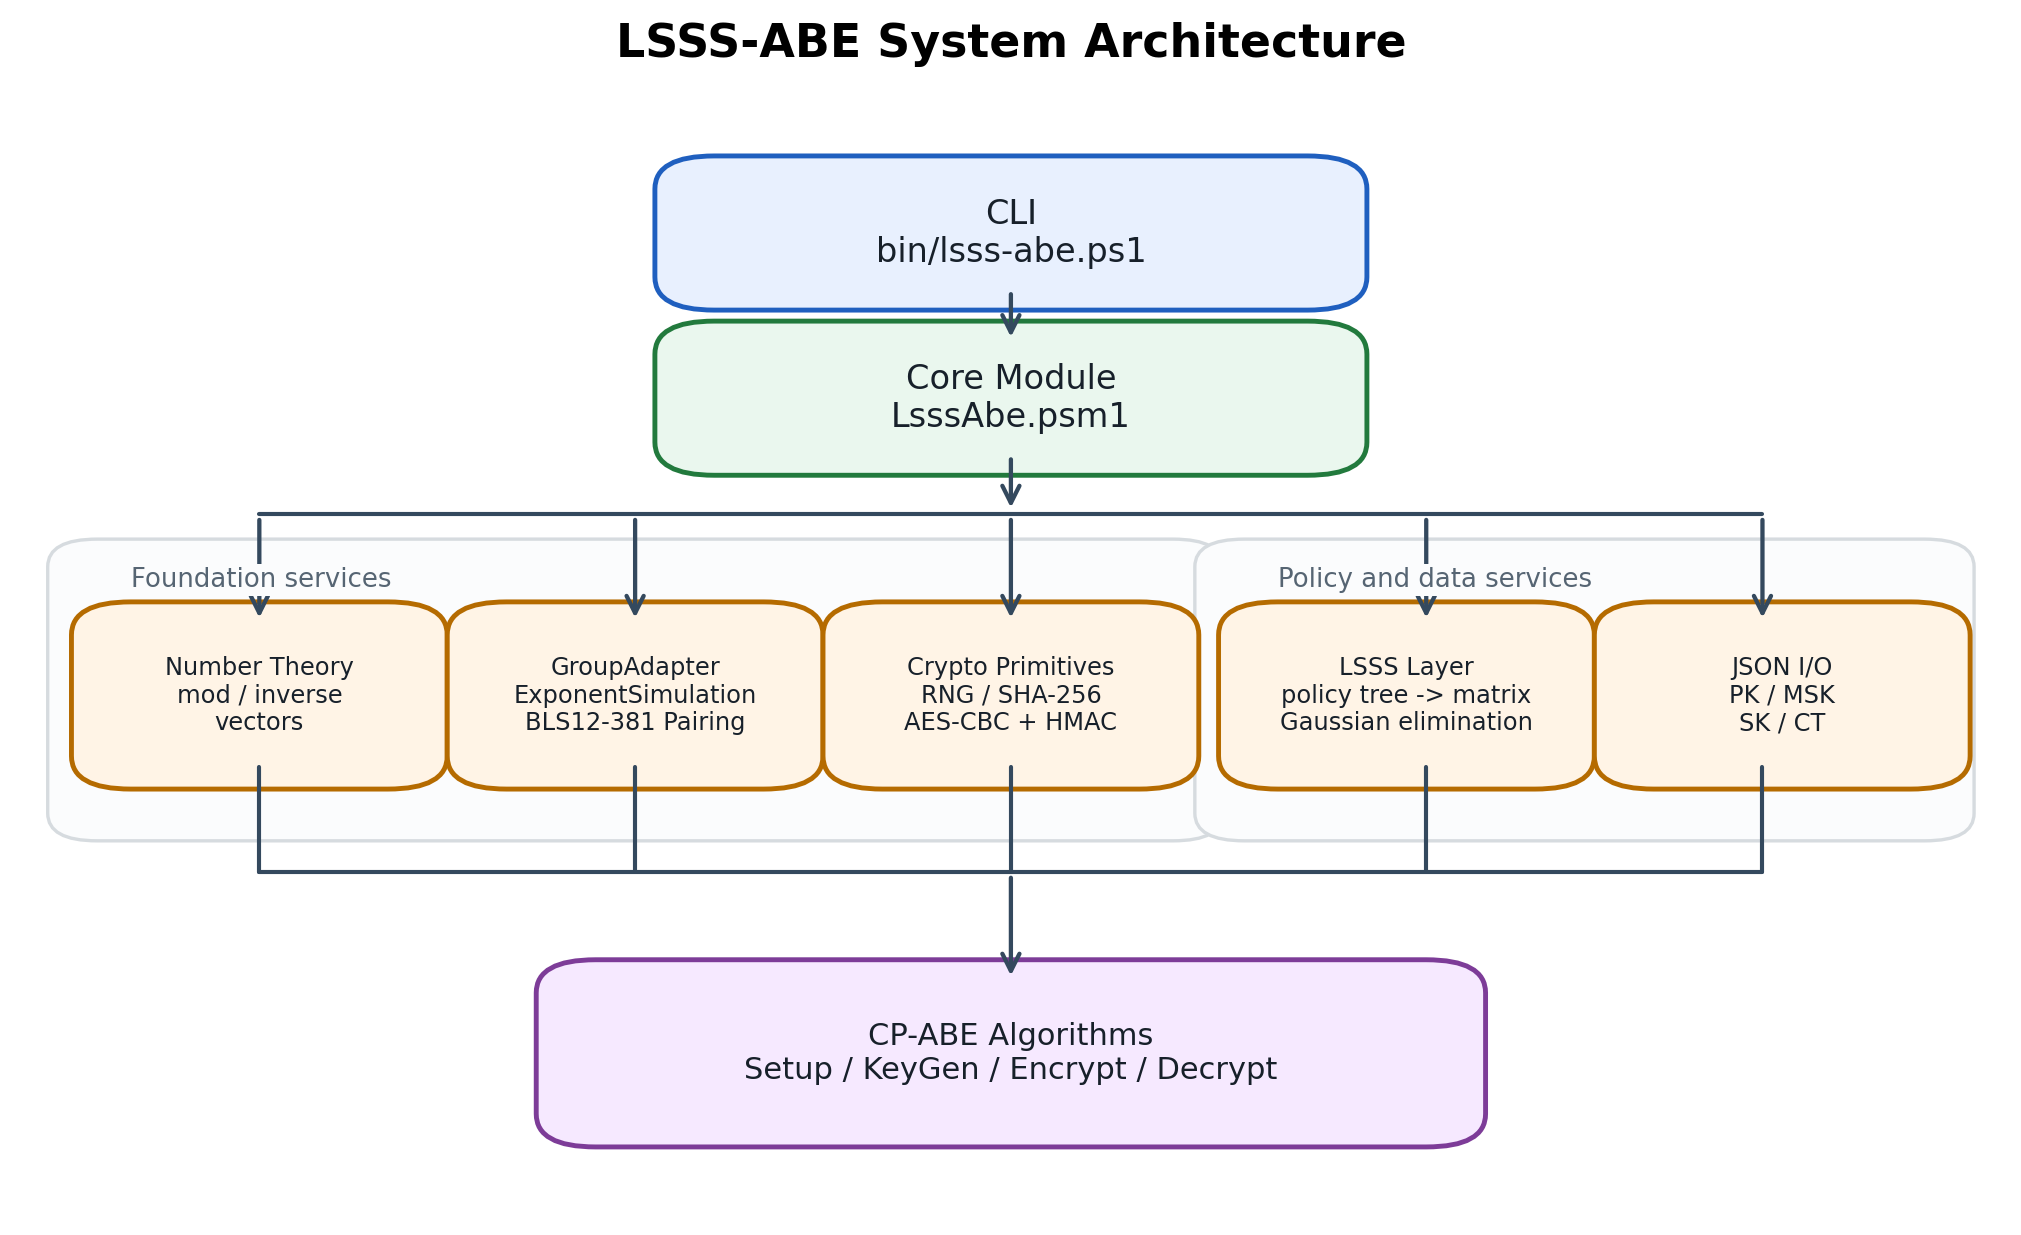
\includegraphics[width=0.95\textwidth]{system_architecture.png}
\caption{系统模块结构图}
\label{fig:system-architecture}
\end{figure}

\section{访问控制树到 LSSS 的构造}

设访问控制树的每个内部节点为阈值门 $k$-of-$d$，对子节点编号为 $1,2,\dots,d$。在每个阈值门处采用 Shamir 风格的多项式分享：为该节点选择次数 $k-1$ 的多项式 $q(x)$，使得该节点持有的份额为 $q(0)$，并将子节点份额设为 $q(1),\dots,q(d)$。

由于多项式求值在域 $\mathbb{Z}_p$ 上是线性的，最终每个叶子份额都可以表示为根秘密 $s$ 与一组随机变量的线性组合。因此可以把每个叶子份额写成：

\[
    \lambda_i = M_i \cdot \mathbf{v},
\]

其中 $\mathbf{v}=(s,r_2,\dots,r_n)$，$M_i$ 为第 $i$ 个叶子对应的系数向量。收集所有叶子的系数向量即可得到 LSSS 矩阵 $M$，并用 $\rho(i)$ 记录第 $i$ 行对应的属性标签。

本项目采用如下列数计算方式：

\[
    n = 1+\sum_{\text{gate }v}(k_v-1).
\]

其中第一列对应根秘密 $s$，每个阈值门额外贡献 $k_v-1$ 个随机维度。对于示例策略 $(A\wedge B)\vee C$，根 OR 门为 $1$-of-$2$，不引入随机维度；内部 AND 门为 $2$-of-$2$，引入一个随机维度。因此最终矩阵列数为 $2$。

这一列数设计体现了“按需引入随机性”的原则。OR 门只需要把父节点份额复制到某个满足的分支，不需要额外随机变量；AND 和一般阈值门则需要通过多项式分享隐藏父节点份额，因此会增加随机维度。这样得到的矩阵既能表达策略，又不会无谓增加列数。

该设计与 Liu、Cao 和 Wong~[4]“直接处理阈值访问树”的思想一致：每个内部节点均作为阈值访问结构参与矩阵生成，而不需要先把阈值策略展开成大量 AND/OR 组合。对于课程题目要求的“使用访问控制树构建 LSSS 矩阵”，这一处理方式使策略树的分支数、层次结构和阈值参数能够直接进入矩阵构造过程，从而区别于只面向固定样例或二叉 AND/OR 公式的实现。

\subsection{访问策略树一般性的体现}

本文所称访问策略树的一般性，主要限定在单调访问结构范围内。也就是说，策略树由属性叶子和阈值门组成，不引入 NOT 这类非单调条件；在这一范围内，系统并不依赖某个固定样例或固定层数的树形结构。策略节点只需要满足两类基本形式：叶子节点保存属性名，内部节点保存阈值 $k$ 与子节点列表。只要 $1\leq k\leq d$，其中 $d$ 为子节点个数，该内部节点就可以作为根节点，也可以出现在任意子树位置；其子节点既可以是属性叶子，也可以继续是阈值门。因此，AND、OR、$2$-of-$3$ 以及更深层的嵌套阈值结构都可以落在同一种访问树表示之下。

这种一般性进一步体现在 LSSS 矩阵构造过程中。转换算法对每个内部节点采用相同的阈值门处理规则：根据节点阈值 $k$ 引入 $k-1$ 个随机维度，以父节点份额作为多项式常数项，再把对子节点编号 $1,\dots,d$ 的求值结果继续向下传递。叶子节点只负责把最终份额向量写入矩阵行，并通过 $\rho$ 记录对应属性。由于递归过程不需要区分“这是 AND 门”“这是 OR 门”或“这是第几层节点”，树的分支数、嵌套深度和阈值取值都由输入策略本身决定。

解密阶段同样没有回到原始访问树上逐个门进行布尔判断，而是根据用户属性集合筛选满足 $\rho(i)\in S$ 的矩阵行，并求解 $M_I^T\omega=e_1$。如果存在重构系数 $\omega$，说明这些行能够恢复根秘密对应的第一维；如果不存在，则属性集合不满足策略。由此，访问策略的满足性被统一转化为线性重构问题。第五章中 $2$-of-$3(D,E,F)$ 的成功与失败测试、重复属性 $X\wedge X$ 测试以及非法策略输入测试，分别从一般阈值门、多行映射同一属性和输入边界三个角度验证了这种设计不是针对示例策略 $(A\wedge B)\vee C$ 的硬编码。

\section{CP-ABE 四个核心算法}

系统包含四个基本算法：Setup、KeyGen、Encrypt 和 Decrypt。它们在命令行中分别对应 \verb|setup|、\verb|keygen|、\verb|encrypt| 和 \verb|decrypt| 四个子命令。

\subsection{Setup}

Setup 生成系统公共参数和主密钥。真实 CP-ABE 中会选择双线性群、生成元和指数。本实验在指数抽象模型下固定素数域 $\mathbb{Z}_p$，并随机选择主密钥指数 $\alpha$ 和 $a$：

\[
    PK=(p,g,g^a,e(g,g)^\alpha),\quad MSK=(\alpha,a).
\]

在 JSON 文件中，$g$ 以指数 $1$ 表示，$g^a$ 存储为 $a$，$e(g,g)^\alpha$ 存储为 $\alpha$。

在真实 pairing 路线中，Setup 使用 BLS12-381 的曲线阶作为标量域，公共参数保存 $g_1\in G_1$、$g_2\in G_2$、$g_1^a$ 以及 $e(g_2,g_1)^\alpha\in G_T$：

\[
    PK=(p,g_1,g_2,g_1^a,e(g_2,g_1)^\alpha),\quad MSK=(\alpha,a).
\]

这些群元素写入 JSON 时会被编码为坐标或系数数组，而不是单个指数值。

Setup 阶段的设计目标是提供后续三个算法共同依赖的公共基础。公共参数中的 $a$ 和 $\alpha$ 会分别进入密文分量和私钥分量，解密时再通过线性组合抵消。主密钥只在 KeyGen 阶段使用，不写入密文，也不参与用户解密命令，这与真实 ABE 系统中“授权中心持有主密钥”的角色划分一致。

\subsection{KeyGen}

KeyGen 为用户属性集合 $S$ 生成私钥。私钥由用户级分量和属性级分量两部分组成：$K$ 与 $L$ 是该用户私钥的全局分量，$K_x$ 是属性 $x\in S$ 对应的分量。这里的下标 $x$ 表示属性索引，因此一个属性集合会对应多个 $K_x$；为避免符号过于繁琐，公式中省略了用户下标，但不同用户重新运行 KeyGen 时会得到不同的具体数值。算法随机选取用户独立随机数 $t$，并生成：

\[
    K=g^\alpha g^{at},\quad L=g^t,\quad K_x=H(x)^t.
\]

上式是论文中常见的群元素写法。本项目采用指数抽象模型保存同一组私钥分量，因此不是再生成一套新的 $K,L,K_x$，而是把这些群元素对应的指数记录下来：

\[
    K=\alpha+at,\quad L=t,\quad K_x=H(x)t.
\]

同一个用户所有属性分量共享同一个 $t$，这体现了抗合谋设计思想：不同用户即使合并属性，也难以把不同随机数 $t$ 的私钥分量拼成一个合法用户的私钥结构。

在本实验实现中，抗合谋性质主要通过公式结构体现，而不是通过完整安全证明体现。报告中保留这一点，是为了说明 KeyGen 不只是为每个属性单独生成一个哈希值，而是把用户级随机数 $t$ 同时绑定到 $K$、$L$ 和所有 $K_x$ 分量中。后续解密公式中的抵消正是依赖这些分量共享同一随机数。

真实 pairing 版沿用这一结构，但分量所在群不同：$K\in G_1$，$L\in G_2$，$K_x\in G_1$。属性哈希 $H(x)$ 由 \verb|hash_to_G1| 产生，使属性名直接映射为 $G_1$ 群元素。该处理比“哈希为标量再写入指数模型”更接近真实配对系统中的属性映射方式。

\subsection{Encrypt}

Encrypt 输入公共参数、访问策略和明文。首先构造 LSSS 矩阵 $(M,\rho)$，然后选择秘密 $s$ 和两个向量：

\[
    \mathbf{v}=(s,r_2,\dots,r_n),\quad
    \mathbf{u}=(0,z_2,\dots,z_n).
\]

对每一行计算：

\[
    \lambda_i=M_i\cdot \mathbf{v},\quad
    w_i=M_i\cdot \mathbf{u}.
\]

其中 $\lambda_i$ 是秘密份额，$w_i$ 是盲化份额。$\mathbf{u}$ 的第一维为 $0$，使得满足策略的线性组合会把盲化项重构为 $0$，从而在解密中抵消。

密文核心分量为：

\[
    C=m+\alpha s,\quad C_0=s,
\]

以及每一行对应的：

\[
    C_i=a\lambda_i-H(\rho(i))w_i,\quad D_i=w_i.
\]

这里的加法、乘法和减法均在模 $p$ 下进行。

真实 pairing 版中，受 CP-ABE 保护的对象是随机 $G_T$ 会话元素 $M$。密文分量对应为：

\[
    C=M\cdot e(g_2,g_1)^{\alpha s},\quad C_0=g_2^s,
\]

以及每一行对应的：

\[
    C_i=(g_1^a)^{\lambda_i}\cdot H(\rho(i))^{-w_i},\quad D_i=g_2^{w_i}.
\]

因此，指数版中的 $C,C_0,C_i,D_i$ 可以看作真实群元素公式在指数层面的投影；pairing 版则直接保存 $G_T$、$G_2$、$G_1$、$G_2$ 中的实际元素。

Encrypt 阶段的两个向量 $\mathbf{v}$ 和 $\mathbf{u}$ 分别承担不同作用。$\mathbf{v}$ 负责分享真正的秘密 $s$，决定满足策略时能恢复出 $\alpha s$；$\mathbf{u}$ 的首项为 $0$，负责生成可抵消的盲化项，防止单个密文行直接泄露份额结构。只有当用户属性集合能够组合出 $(1,0,\dots,0)$ 时，盲化项才会在线性重构中同时消去。

实验三课件~[1]中 Waters 2011 加密步骤强调对访问矩阵每一行计算 $\lambda_i=\mathbf{v}\cdot M_i$；Waters~[3]则把密文与 LSSS 访问结构 $(M,\rho)$ 绑定。本项目在此基础上额外保留 $\mathbf{u}$ 盲化向量，是为了在指数抽象模型中呈现解密抵消过程：满足策略时 $\mathbf{v}$ 的第一维恢复 $s$，而 $\mathbf{u}$ 的第一维为 $0$，因此盲化项随同线性重构被消去。

\subsection{Decrypt}

Decrypt 输入公共参数、用户私钥和密文。首先筛选所有满足 $\rho(i)\in S$ 的行，构造行集合 $I$。然后求解：

\[
    M_I^T\omega=e_1,
\]

其中 $e_1=(1,0,\dots,0)^T$。如果该方程无解，说明用户属性集合不能满足策略，算法抛出错误并拒绝解密。

如果方程有解，则计算：

\[
\begin{aligned}
A &= \sum_{i\in I}\omega_i(C_iL+D_iK_{\rho(i)})\\
  &= \sum_{i\in I}\omega_i((a\lambda_i-H(\rho(i))w_i)t+w_iH(\rho(i))t)\\
  &= at\sum_{i\in I}\omega_i\lambda_i\\
  &= ats.
\end{aligned}
\]

再计算：

\[
    B=C_0K-A=s(\alpha+at)-ats=\alpha s,
\]

最终恢复：

\[
    m=C-B.
\]

恢复出的 $m$ 用于派生对称密钥，进而验证 HMAC 并解密 AES-CBC 载荷。

在真实 pairing 版中，解密端计算：

\[
\prod_{i\in I}\left(e(L,C_i)\cdot e(D_i,K_{\rho(i)})\right)^{\omega_i}
    = e(g_2,g_1)^{ats},
\]

再用

\[
    e(C_0,K)=e(g_2,g_1)^{\alpha s+ats}
\]

消去 $ats$，得到 $e(g_2,g_1)^{\alpha s}$。随后从 $C$ 中除去该遮蔽项即可恢复 $G_T$ 会话元素，并由该元素派生 AES/HMAC 密钥。

Decrypt 阶段的失败路径同样重要。如果求不出 $\omega$，程序不会尝试“部分解密”，而是立即抛出不满足策略的错误。这使访问控制语义和线性方程求解结果保持一致：有解代表满足策略，无解代表拒绝访问。后续实验中的 $\{A\}$ 和 $\{D\}$ 两个失败场景都用于验证这一点。

Waters~[3]对 Decrypt 的描述中，满足策略的属性集合对应行集合 $I=\{i:\rho(i)\in S\}$，并存在一组常数使得这些行可以线性恢复秘密。实现时选择直接求解 $M_I^T\omega=e_1$，能够把这一理论条件变成可执行的判定过程。这也是本项目没有单独写树满足性递归判断的原因：矩阵可解性已经完整表达了访问结构语义。

\section{数据流设计}

图 \ref{fig:encrypt-decrypt-flow} 展示了系统的主要数据流。加密端从策略 JSON 和明文出发，生成密文 JSON；解密端从密文 JSON 和用户私钥出发，先求解 LSSS 重构系数，再恢复对称密钥并输出明文。

数据流设计中特别保留了中间结构：密文不仅保存对称密文，还保存策略树、矩阵 $M$ 和映射 $\rho$。这样做会使密文 JSON 更大，但能够把“访问树已经被转换为矩阵”这一过程固化在实验文件中，也使失败场景能够回到矩阵行和属性映射层面分析原因。

\begin{figure}[H]
\centering
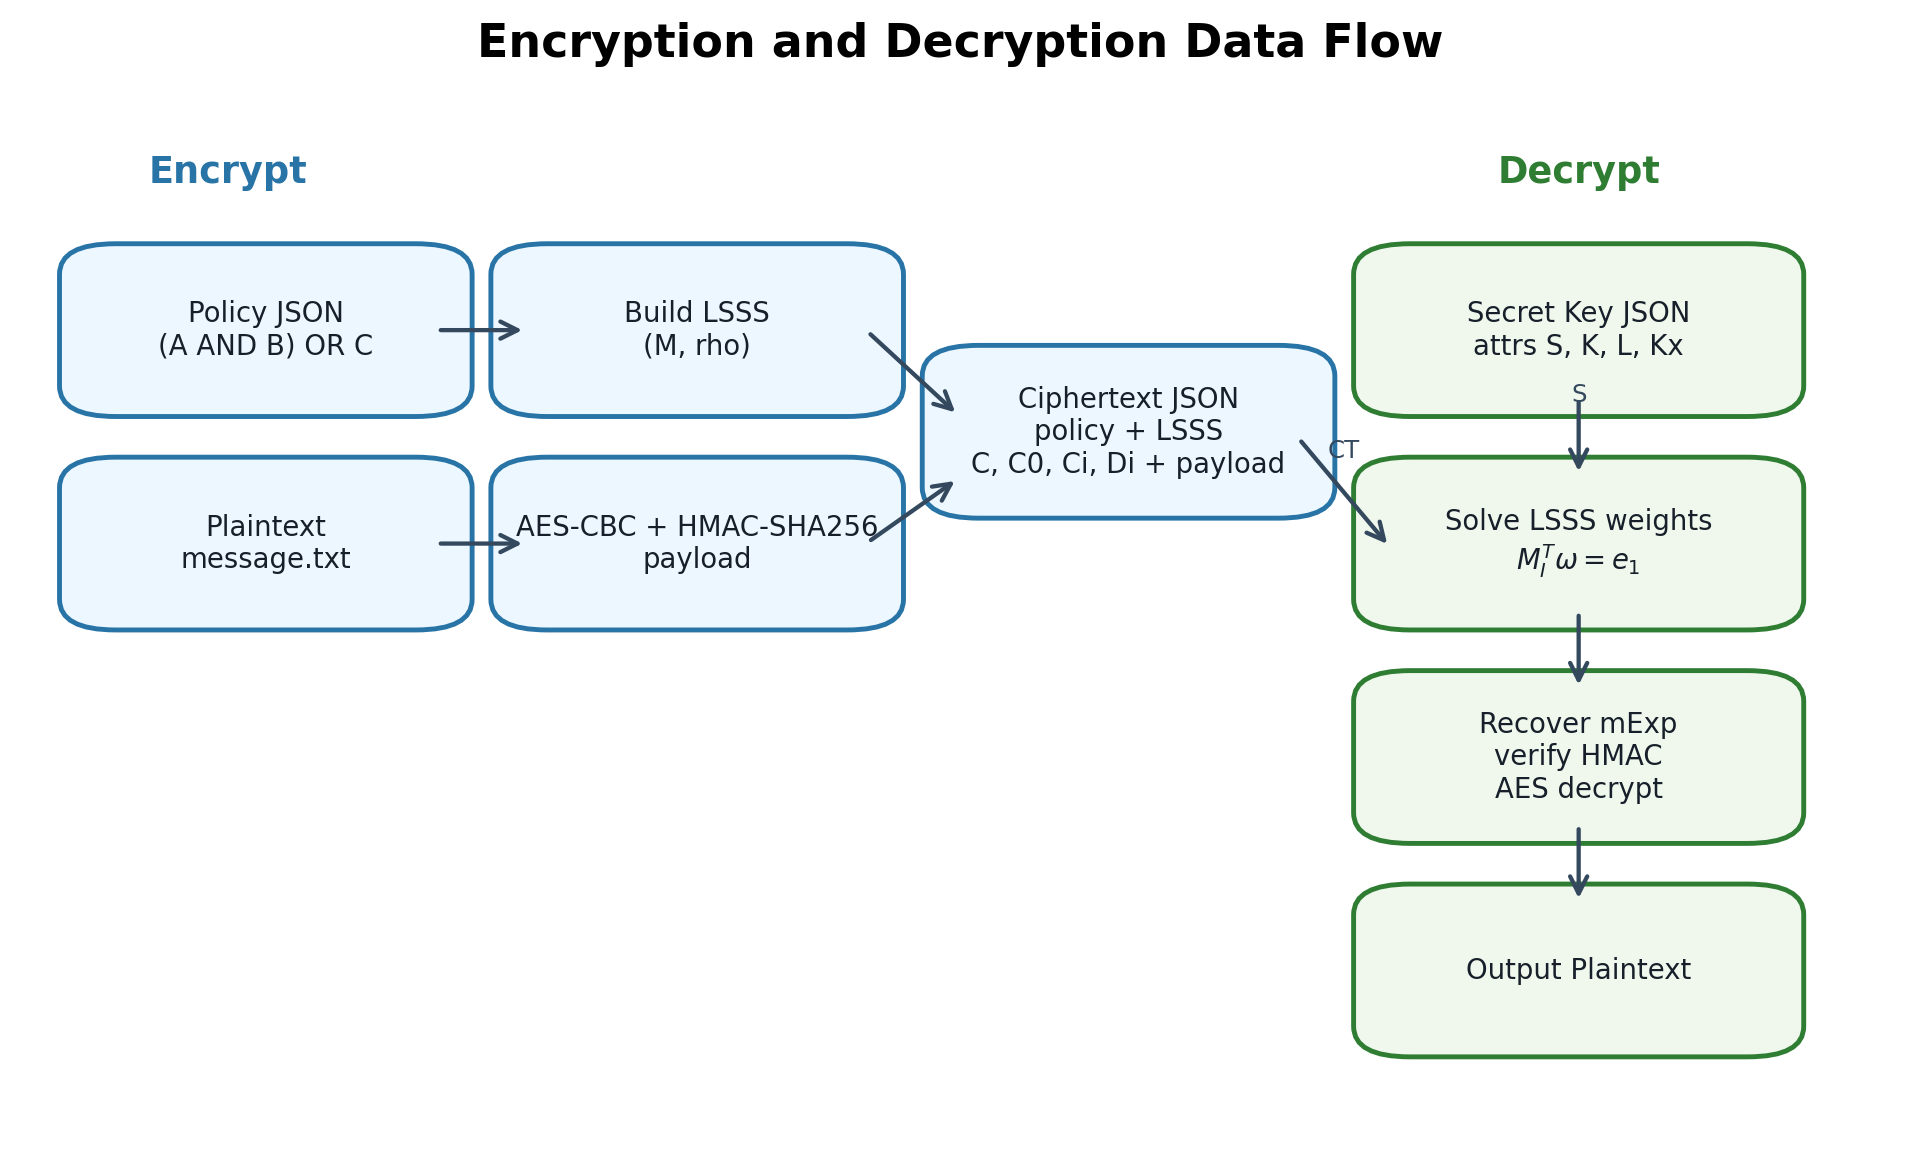
\includegraphics[width=0.95\textwidth]{encrypt_decrypt_flow.png}
\caption{加密与解密数据流}
\label{fig:encrypt-decrypt-flow}
\end{figure}

\section{工程化接口设计}

为便于实验展示与复现，系统提供命令行接口：

\begin{table}[H]
\centering
\caption{命令行接口}
\begin{tabular}{p{0.18\textwidth} p{0.70\textwidth}}
\toprule
命令 & 作用 \\
\midrule
\verb|setup| & 生成公共参数 \verb|public.json| 和主密钥 \verb|master.json|。\\
\verb|keygen| & 输入公共参数、主密钥和属性集合，生成用户私钥 JSON。\\
\verb|encrypt| & 输入公共参数、策略 JSON 和明文文件，输出密文 JSON。\\
\verb|decrypt| & 输入公共参数、用户私钥和密文 JSON，输出恢复后的明文文件。\\
\verb|-Adapter| \verb|pairing| & 启用 BLS12-381 真实 pairing 后端。\\
\bottomrule
\end{tabular}
\end{table}

这种 CLI 设计使每个算法阶段都保留单独的文件结果，便于在实验分析中追踪 Setup、KeyGen、Encrypt 和 Decrypt 的状态变化。JSON 格式虽然不如二进制编码紧凑，但具有可读性强、便于调试、便于展示矩阵和中间分量的优点。

与只提供函数接口相比，CLI 使实验过程具有更清晰的阶段边界。逐条命令和烟雾测试脚本都会在 \path{tests/artifacts} 目录下留下公共参数、主密钥、用户私钥、密文和解密输出，这些文件与报告中的字段说明可以相互对应。

\section{安全性边界与实现取舍}

本节的安全性边界主要用于明确本实验设计所覆盖的问题范围。本文实现的核心目标是验证“访问控制树能够被转换为 LSSS 矩阵，并进一步嵌入 CP-ABE 四算法流程”这一主线。因此，报告中的安全性讨论并不等同于完整 CP-ABE 论文中的安全证明，而是围绕访问结构正确性、代数重构正确性、密文载荷完整性和实现边界展开。这样处理可以避免把“算法流程能够正确运行”和“方案已经满足标准模型或选择明文安全证明”混为一谈。

在指数抽象模型中，真实群元素被表示为指数，群乘法、幂运算和双线性对分别对应指数加法、指数乘法和指数乘积。该模型保留了 CP-ABE 解密公式中最关键的代数关系：满足访问结构的属性集合能够通过重构系数恢复秘密 $s$，并使盲化项在线性组合中抵消；不满足访问结构的属性集合无法求得 $M_I^T\omega=e_1$ 的解，因此不能进入消息恢复流程。真实 pairing 路线进一步把这些关系放入 BLS12-381 的群元素和配对运算中执行，能够检验群元素序列化、配对调用和 $G_T$ 密钥派生是否与访问结构逻辑正确衔接。

同时，即使接入真实 pairing 库，报告中的安全性讨论仍不能等同于完整论文安全证明。真实 CP-ABE 方案中的安全性通常依赖素数阶配对友好曲线、随机预言机或标准模型假设、群元素序列化约束、严格随机数生成过程以及与论文完全一致的算法分量。真实 pairing 路线已经覆盖真实群元素、哈希到群、配对和基本反序列化检查，但仍需把“可运行的真实群实现”和“满足某篇论文安全模型的完整实现”区分开。

\begin{table}[H]
\centering
\caption{本实验实现的安全性边界}
\begin{tabular}{>{\raggedright\arraybackslash}p{0.20\textwidth} >{\raggedright\arraybackslash}p{0.35\textwidth} >{\raggedright\arraybackslash}p{0.33\textwidth}}
\toprule
分析对象 & 本实验覆盖内容 & 边界说明 \\
\midrule
访问策略 & 支持属性叶子、AND/OR 和一般阈值门，并由访问树生成 LSSS 矩阵 & 限定于单调访问结构，不包含 NOT 等非单调条件 \\
解密判定 & 通过 $M_I^T\omega=e_1$ 判断属性集合是否满足策略 & 正确性依赖矩阵构造与有限域线性求解实现 \\
代数抵消 & 在指数抽象模型中验证 $\lambda_i$、$w_i$、$K$、$L$、$K_x$ 的抵消关系，并在 pairing 版中用真实配对复核同一访问逻辑 & pairing 版提升了实现真实性，但仍不等同于形式化安全证明 \\
载荷保护 & 使用 AES-CBC 加密明文，并用 HMAC-SHA256 验证 IV 与密文完整性 & 对称层保护文件载荷，不改变 CP-ABE 访问结构语义 \\
输入边界 & 对非法策略、重复属性和特殊属性名进行测试 & 工程健壮性测试不等同于形式化安全证明 \\
\bottomrule
\end{tabular}
\end{table}

从实现取舍看，本文先建立了相对独立的群运算抽象层，再在同一 \verb|Project| 中接入真实 BLS12-381 后端。这样做使访问树解析、LSSS 矩阵生成、有限域高斯消元、密文 JSON 结构和 CLI 流程能够先被完整验证，再逐步替换底层群元素生成、群运算、配对、哈希到群和序列化部分。实际接入结果也说明，访问树到矩阵、行集合筛选和重构系数求解等逻辑可以保持稳定，变化最大的部分集中在群元素表示和密文/私钥 JSON 编码上。

这一边界划分也决定了实验结果分析的侧重点。对于本项目，关键分析对象不是群元素计算性能或安全证明强度，而是策略语义是否被正确转换为矩阵，满足策略的属性集合是否能够恢复消息指数，不满足策略的属性集合是否被拒绝，以及密文载荷被篡改时是否无法输出明文。第五章设计的成功解密、失败解密、一般阈值门、重复属性、非法策略和密文篡改测试，正是围绕这些边界进行验证。

Riepel 和 Wee 提出的 FABEO 方案~[5]表明，真实 ABE 方案还会进一步关注自适应安全、多密文安全、配对次数、群元素大小以及属性多次出现带来的效率与安全权衡。与这些研究目标相比，本文的方案设计更侧重课程实验要求中的访问控制树、LSSS 矩阵和 CP-ABE 基本流程。真实 pairing 路线提高了底层密码运算的真实性，但本文仍把结论限定在可由实现和实验直接支撑的范围内。

\chapter{系统实现}

\section{实现语言与运行环境}

本实验实现使用 Windows PowerShell 脚本与模块组织代码。选择 PowerShell 的主要原因是 Windows 系统默认提供运行环境，并且能够调用 .NET 标准库中的大整数、随机数、哈希和对称加密组件。同一 \verb|Project| 工程在此基础上增加 Python 后端，用于调用真实 BLS12-381 pairing 库。系统源码主要位于：

\begin{itemize}
    \item \verb|Project/src/LsssAbe/LsssAbe.psm1|：核心模块。
    \item \verb|Project/bin/lsss-abe.ps1|：命令行入口。
    \item \verb|Project/tests/smoke.ps1|：烟雾测试。
    \item \verb|Project/src/LsssAbe/pairing_backend.py|：真实 BLS12-381 pairing 后端。
    \item \verb|Project/tests/smoke_pairing.ps1|：真实 pairing 版烟雾测试。
\end{itemize}

核心模块没有依赖第三方包，主要使用以下 .NET 类型：

\begin{table}[H]
\centering
\caption{实现中使用的主要 .NET 组件}
\begin{tabular}{p{0.35\textwidth} p{0.52\textwidth}}
\toprule
组件 & 用途 \\
\midrule
\verb|System.Numerics.BigInteger| & 表示模 $p$ 下的大整数和指数。\\
\verb|RandomNumberGenerator| & 生成密码学安全随机字节。\\
\verb|SHA256| & 将属性名和消息指数映射到固定长度摘要。\\
\verb|Aes| & 使用 AES-CBC 加密明文载荷。\\
\verb|HMACSHA256| & 对 IV 和密文进行完整性认证。\\
\bottomrule
\end{tabular}
\end{table}

真实 pairing 后端运行在 \verb|E:\WHU\Kinding_Plan\LSSS-ABE\env| 环境中，主要依赖如表 \ref{tab:python-pairing-deps} 所示。

\begin{table}[H]
\centering
\caption{真实 pairing 后端使用的 Python 组件}
\label{tab:python-pairing-deps}
\begin{tabular}{p{0.30\textwidth} p{0.58\textwidth}}
\toprule
组件 & 用途 \\
\midrule
\verb|py-ecc| & 提供 BLS12-381 的 $G_1/G_2/G_T/\mathbb{Z}_p$、标量乘法、群加法、哈希到 $G_1$ 和 \verb|pairing|。\\
\verb|pycryptodome| & 在真实 pairing 后端中实现 AES-CBC 加密、PKCS7 填充和 HMAC 所需基础能力。\\
\verb|secrets|、\verb|hashlib|、\verb|hmac| & 提供随机标量采样、SHA-256 摘要和认证标签比较。\\
\bottomrule
\end{tabular}
\end{table}

\section{模块结构}

核心模块可以分为六类函数：

\begin{enumerate}
    \item 数论工具：模运算、模逆、快速幂、向量加法、向量数乘和内积。
    \item 群运算适配器：封装随机标量、属性哈希、群加减乘和配对接口。
    \item 密码原语：随机数、哈希、AES-CBC-HMAC。
    \item 策略与 LSSS：策略树读取、随机维度统计、门索引分配、矩阵构造。
    \item 线性重构：从用户属性筛选行并用高斯消元求 $\omega$。
    \item CP-ABE 主算法：Setup、KeyGen、Encrypt、Decrypt。
\end{enumerate}

这样的分组虽然都位于同一个 PowerShell 模块文件中，但逻辑边界比较清晰。CLI 脚本只调用导出的主函数，不直接操作内部数学细节。

在实现时，核心模块没有进一步拆成多个文件，主要是为了降低实验复现时的路径复杂度。虽然文件较长，但函数命名保持了统一前缀 \verb|LsssAbe|，并按照“工具函数在前、算法函数在后、导出函数最后”的顺序组织。Setup、KeyGen、Encrypt 和 Decrypt 四个导出主函数集中呈现算法主流程，访问树到 LSSS 矩阵的转换函数则集中呈现矩阵构造逻辑。

这种组织方式也对应实验三课件~[1]中的算法分块：先准备底层群运算和随机数，再实现 KeyGen、Encrypt、Decrypt 等主算法。基础实现把真实群运算替换为模 $p$ 指数运算，把 Charm-Crypto 依赖替换为 PowerShell 与 .NET 标准库，从而使实验环境更容易复现；真实 pairing 路线则通过 Python 后端补回真实 pairing 运算，用于检查同一 LSSS 主线在真实曲线群元素上的运行情况。

\section{群运算适配器设计}

为使当前实验实现具备向真实双线性群迁移的边界，核心模块新增了群运算适配器层。现有默认适配器为 \verb|ExponentSimulation|，它仍然使用整数指数表示群元素：群乘法对应指数加法，配对对应指数乘法。因此，当前密文格式和实验行为保持不变，但 Setup、KeyGen、Encrypt 和 Decrypt 不再直接散落书写底层指数运算，而是通过适配器函数完成。

适配器层的核心接口包括：

\begin{itemize}
    \item \verb|New-LsssAbeGroupRandomScalar|：生成 $\mathbb{Z}_p$ 中的随机标量。
    \item \verb|New-LsssAbeGroupHashAttribute|：把属性字符串映射为当前指数抽象模型中的标量。
    \item \verb|Invoke-LsssAbeGroupAdd|、\verb|Invoke-LsssAbeGroupSub|、\verb|Invoke-LsssAbeGroupMul|：封装群指数模型下的加减乘。
    \item \verb|Invoke-LsssAbeGroupPair|：封装配对接口；在当前指数模型中返回两个指数的乘积。
\end{itemize}

关键代码节选如下：

\begin{lstlisting}[language=bash,caption={指数抽象群运算适配器关键代码}]
function New-LsssAbeExponentGroupAdapter {
    param([Parameter(Mandatory)][System.Numerics.BigInteger]$p)

    [pscustomobject]@{
        name = "ExponentSimulation"
        scalarModulus = $p
        supportsRealPairing = $false
    }
}

function Invoke-LsssAbeGroupPair {
    param(
        [Parameter(Mandatory)][object]$Group,
        [Parameter(Mandatory)][System.Numerics.BigInteger]$Left,
        [Parameter(Mandatory)][System.Numerics.BigInteger]$Right
    )

    Invoke-LsssAbeGroupMul -Group $Group -a $Left -b $Right
}
\end{lstlisting}

在当前 \verb|Project| 中，命令行入口新增 \verb|-Adapter pairing| 参数。当该参数被启用时，PowerShell 不再调用指数抽象模块中的四个主函数，而是把 setup、keygen、encrypt、decrypt 命令转发给 Python 后端 \verb|pairing_backend.py|。这种桥接方式保持了 CLI 使用习惯，同时避免在 PowerShell 中手动实现复杂的椭圆曲线群元素运算。

\begin{lstlisting}[language=bash,caption={CLI 中转发真实 pairing 后端的关键代码}]
if ($Adapter -eq "pairing") {
    switch ($Command) {
        "setup" {
            Invoke-PairingBackend -BackendArgs @("setup", "--out-dir", $OutDir)
            break
        }
        "keygen" {
            Invoke-PairingBackend -BackendArgs @("keygen", "--pub", $Pub,
                "--msk", $Msk, "--attrs", $Attrs, "--out-dir", $OutDir)
            break
        }
        "encrypt" {
            Invoke-PairingBackend -BackendArgs @("encrypt", "--pub", $Pub,
                "--policy", $Policy, "--input", $In, "--output", $Out)
            break
        }
        "decrypt" {
            Invoke-PairingBackend -BackendArgs @("decrypt", "--pub", $Pub,
                "--sk", $Sk, "--input", $In, "--output", $Out)
            break
        }
    }
    return
}
\end{lstlisting}

\subsection{真实 pairing 后端}

真实 pairing 后端的核心职责是把 CP-ABE 中的群元素计算放到 BLS12-381 上执行。后端从 \verb|py_ecc.optimized_bls12_381| 导入 $G_1$、$G_2$、$G_T$、曲线阶、标量乘法、群加法、逆元和配对函数，并从 \verb|py_ecc.bls.hash_to_curve| 导入 \verb|hash_to_G1|。关键导入如下：

\begin{lstlisting}[language=Python,caption={真实 pairing 后端关键导入}]
from py_ecc.bls.hash_to_curve import hash_to_G1
from py_ecc.optimized_bls12_381 import (
    G1, G2, Z1, Z2, FQ, FQ2, FQ12,
    add, multiply, neg, pairing,
    curve_order, is_inf, is_on_curve,
)
\end{lstlisting}

Setup 阶段在真实后端中选择随机标量 $\alpha$ 和 $a$，生成 $g_1^a$ 和 $e(g_2,g_1)^\alpha$。Encrypt 阶段为每个矩阵行生成 $C_i\in G_1$ 和 $D_i\in G_2$，Decrypt 阶段调用 \verb|pairing| 计算 $e(L,C_i)$、$e(D_i,K_{\rho(i)})$ 和 $e(C_0,K)$。核心代码如下：

\begin{lstlisting}[language=Python,caption={真实 pairing 后端的加解密核心片段}]
egg_alpha = pairing(G2, G1) ** alpha

ci = add(multiply(g1_a, lambdas[i]),
         neg(multiply(h_attr, blind[i])))
di = multiply(g2, blind[i])

term = pairing(L, Ci[row_index]) * pairing(Di[row_index], Kx[attr])
A *= term ** weights["omega"][pos]
masked = pairing(C0, K) * A.inv()
message_gt = C * masked.inv()
\end{lstlisting}

后端还实现了群元素 JSON 编码与反序列化检查。对于 $G_1$ 和 $G_2$ 点，程序会检查曲线成员关系，并用曲线阶乘法检查子群成员关系；对于 $G_T$ 元素，程序检查系数数量是否为 12。该处理使密钥和密文不再只是整数文件，而是包含真实曲线点和目标群元素的结构化 JSON。

\section{数据结构设计}

\subsection{访问控制树}

策略采用 JSON 表示。叶子节点包含 \verb|attr| 字段：

\begin{lstlisting}[caption={叶子属性节点示例}]
{ "attr": "A" }
\end{lstlisting}

内部节点包含阈值 \verb|k| 和子节点数组 \verb|children|：

\begin{lstlisting}[caption={阈值门节点示例}]
{
  "k": 2,
  "children": [
    { "attr": "A" },
    { "attr": "B" }
  ]
}
\end{lstlisting}

示例策略 $(A\wedge B)\vee C$ 写成：

\begin{lstlisting}[caption={示例访问策略 JSON}]
{
  "k": 1,
  "children": [
    {
      "k": 2,
      "children": [
        { "attr": "A" },
        { "attr": "B" }
      ]
    },
    { "attr": "C" }
  ]
}
\end{lstlisting}

策略对象进入矩阵构造前会先经过递归校验。该校验把属性叶子和阈值门分开处理，能够在加密前拒绝空属性、缺失阈值、空子节点、非法阈值以及叶子节点错误携带子节点等情况。关键代码节选如下：

\begin{lstlisting}[language=bash,caption={访问策略递归校验关键代码}]
function Assert-LsssAbePolicyNode {
    param([Parameter(Mandatory)][AllowNull()][object]$Node)

    if ($null -eq $Node) { throw "Invalid policy node: node must not be null." }

    $attr = Get-LsssAbeProp -Obj $Node -Name "attr"
    $childrenValue = Get-LsssAbeProp -Obj $Node -Name "children"

    if ($null -ne $attr) {
        if (-not ($attr -is [string])) { throw "Invalid policy leaf: attr must be a string." }
        if ([string]::IsNullOrWhiteSpace([string]$attr)) { throw "Invalid policy leaf: attr must not be empty." }
        if ($null -ne $childrenValue) { throw "Invalid policy node: leaf must not also define children." }
        return
    }

    $kValue = Get-LsssAbeProp -Obj $Node -Name "k"
    if ($null -eq $kValue) { throw "Invalid policy gate: missing k." }
    if ($null -eq $childrenValue) { throw "Invalid policy gate: missing children." }

    $children = @($childrenValue)
    if ($children.Length -lt 1) { throw "Invalid policy gate: children must not be empty." }
    if (-not ($kValue -is [byte] -or $kValue -is [int16] -or $kValue -is [int32] -or $kValue -is [int64])) {
        throw "Invalid policy gate: k must be an integer."
    }
    $k = [int]$kValue
    if ($k -lt 1) { throw "Invalid policy gate: k must be at least 1." }
    if ($k -gt $children.Length) { throw "Invalid policy gate: k must not exceed child count." }

    foreach ($c in $children) { Assert-LsssAbePolicyNode -Node $c }
}
\end{lstlisting}

这一段校验代码的意义在于把错误尽量前移。如果非法策略直接进入矩阵构造过程，后续错误可能表现为数组越界、空对象访问或线性代数维度不一致，定位成本较高。现在系统在加密前即可给出 \verb|Invalid policy| 相关错误，实验中的非法策略输入场景也正是验证这一点。

\subsection{LSSS 表示}

构造结果包含矩阵 $M$ 和映射 $\rho$。在内存中，矩阵行是 \verb|BigInteger[]|；写入 JSON 时，每个整数转为字符串，避免大整数在 JSON 解析时发生精度损失。

图 \ref{fig:policy-lsss-matrix} 展示了示例策略到矩阵的转换结果。

\begin{figure}[H]
\centering
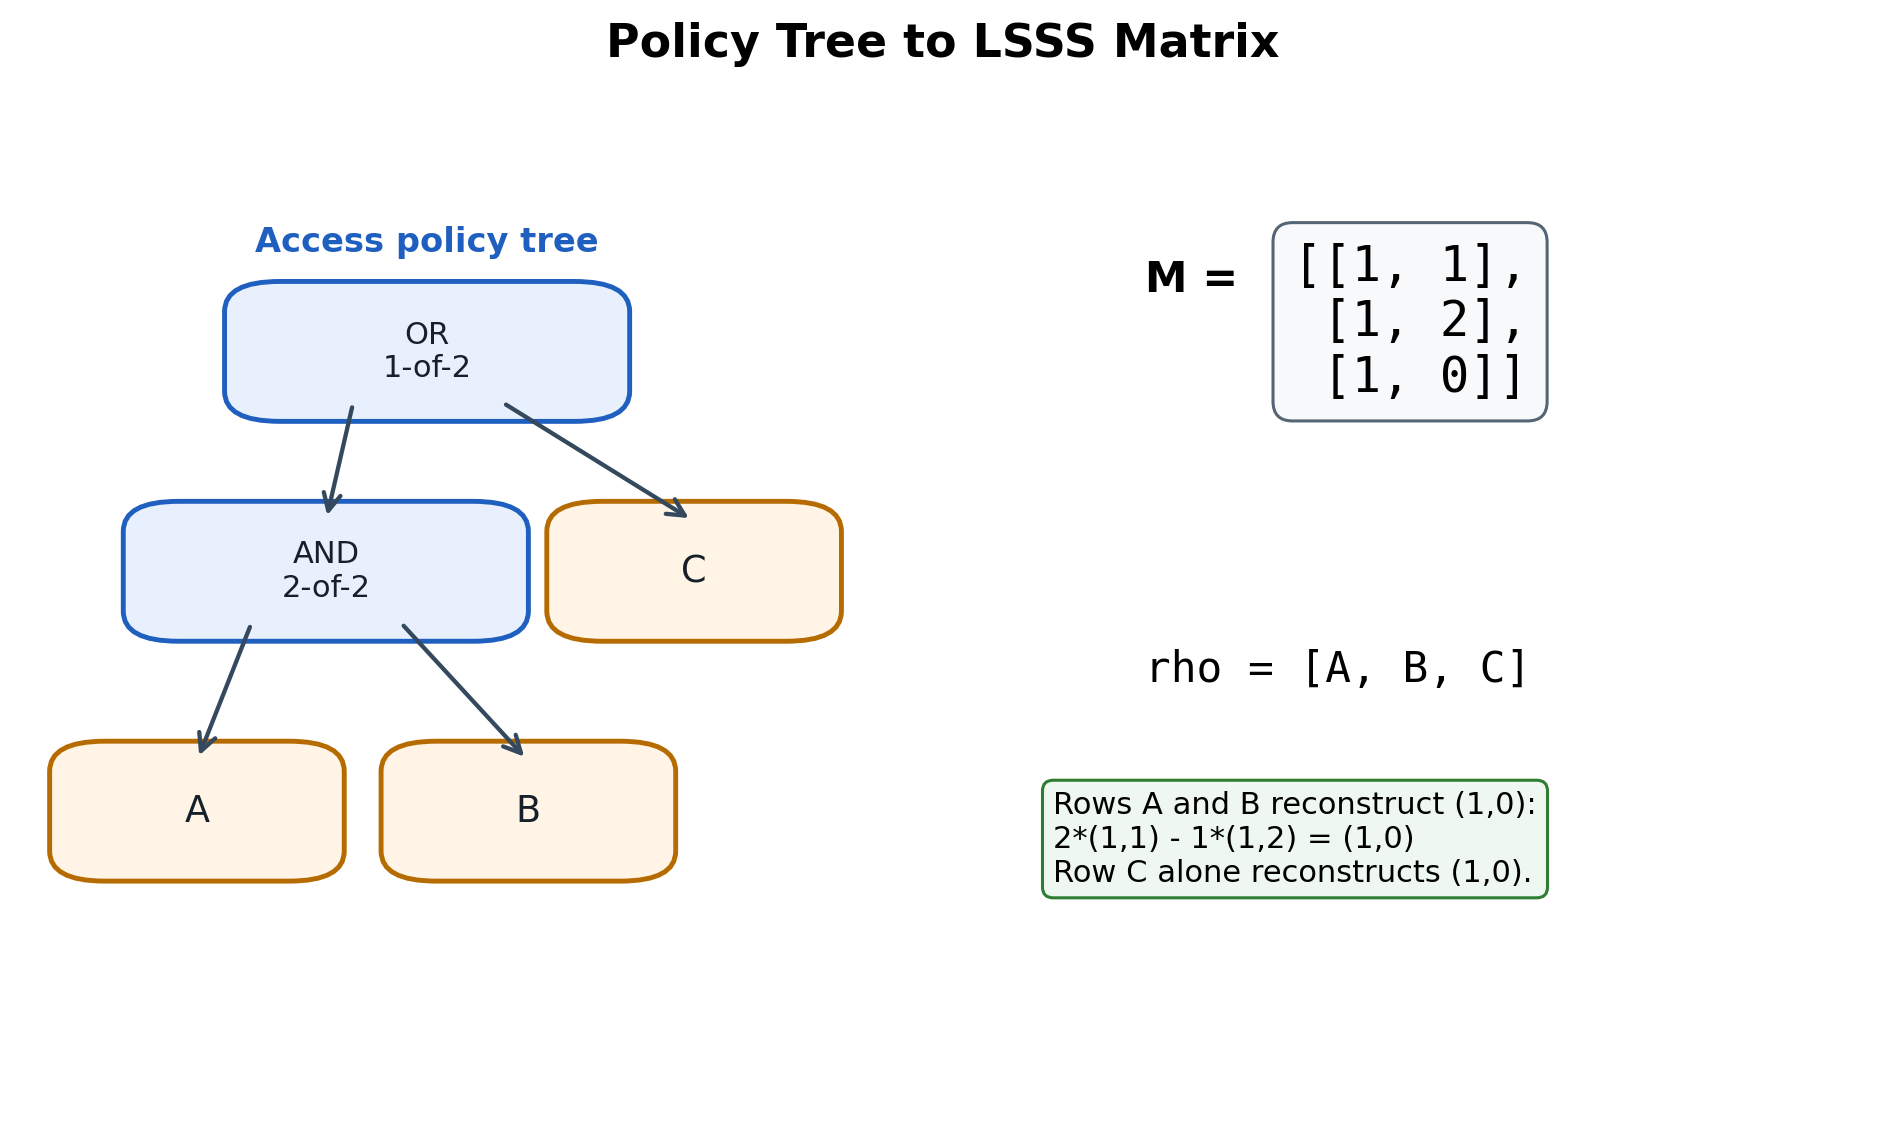
\includegraphics[width=0.95\textwidth]{policy_lsss_matrix.png}
\caption{示例策略到 LSSS 矩阵的转换}
\label{fig:policy-lsss-matrix}
\end{figure}

图 \ref{fig:ct-json-lsss-screenshot} 展示了实际密文文件 \verb|ct.json| 中的 \verb|lsss| 字段。密文不仅保存对称加密载荷，也保存由访问控制树生成的矩阵 $M$ 和行属性映射 $\rho$，使矩阵结构能够与前文的策略转换结果相互对应。

\begin{figure}[H]
\centering
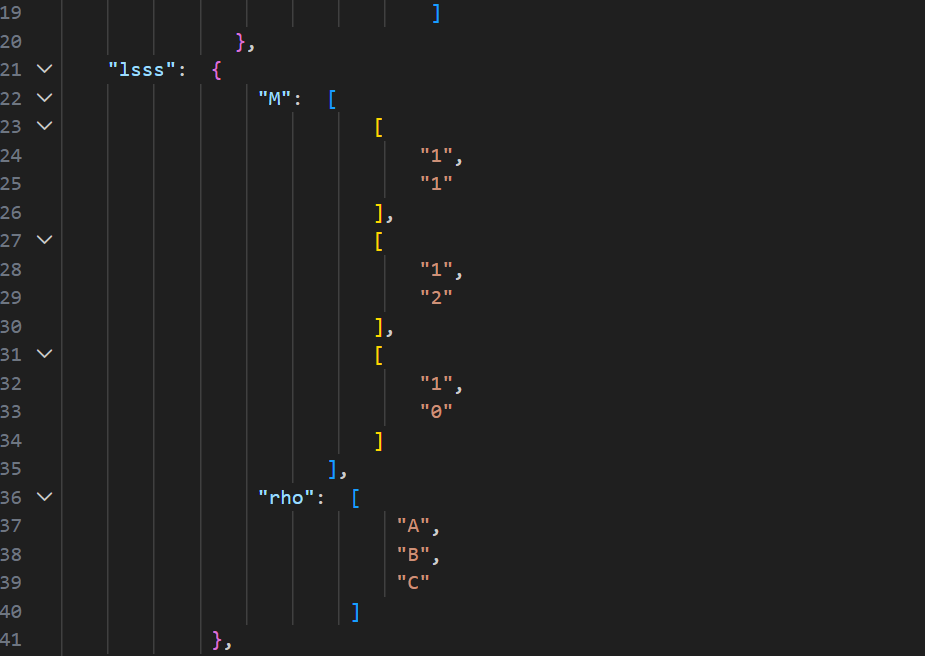
\includegraphics[width=0.85\textwidth]{ct_json_M_rho.png}
\caption{密文 ct.json 中 LSSS 矩阵与 $\rho$ 映射截图}
\label{fig:ct-json-lsss-screenshot}
\end{figure}

\subsection{密钥与密文}

公共参数、主密钥、用户私钥和密文都使用 JSON 存储。这样做的优点是便于人工检查和报告分析。例如密文中不仅包含 CP-ABE 分量，还包含策略树、LSSS 矩阵、属性映射和对称加密载荷。

JSON 存储还有一个现实好处：它让每个阶段的输出都能成为下一阶段的输入文件。Setup 输出的 \verb|public.json| 和 \verb|master.json| 被 KeyGen 和 Encrypt 使用；KeyGen 输出的 \verb|sk_*.json| 被 Decrypt 使用；Encrypt 输出的密文 JSON 同时携带策略和密文分量。这样整个实验过程可以被拆成一组清晰的命令，而不是隐藏在一个不可观察的内存流程中。

\begin{table}[H]
\centering
\caption{主要 JSON 对象字段}
\begin{tabular}{p{0.20\textwidth} p{0.25\textwidth} p{0.45\textwidth}}
\toprule
对象 & 字段 & 含义 \\
\midrule
公共参数 & \verb|p|、\verb|g|、\verb|ga|、\verb|egg_alpha| & 素数模数、生成元指数、公钥指数分量。\\
主密钥 & \verb|alpha|、\verb|a| & 主密钥指数。\\
用户私钥 & \verb|attrs|、\verb|K|、\verb|L|、\verb|Kx| & 用户属性集合和属性密钥分量。\\
密文 & \verb|policy|、\verb|lsss|、\verb|C|、\verb|C0|、\verb|Ci|、\verb|Di|、\verb|payload| & 策略、矩阵、CP-ABE 分量和对称密文载荷。\\
\bottomrule
\end{tabular}
\end{table}

真实 pairing 版沿用相同的高层字段名称，但字段内容不同。例如公共参数中的 \verb|g1_a| 保存 $G_1$ 点，\verb|egg_alpha| 保存 $G_T$ 元素；密文中的 \verb|C| 是 $G_T$ 元素，\verb|C0| 和 \verb|Di| 是 $G_2$ 点，\verb|Ci| 是 $G_1$ 点。因此，指数版和 pairing 版的 JSON 文件不能混用。保留相同字段语义的好处是报告中的算法结构仍然一致，而字段内部编码反映了底层群实现的差异。

\section{访问控制树到 LSSS 的实现}

实现树到矩阵转换的主函数是 \verb|ConvertTo-LsssAbeLsssFromPolicy|。其步骤如下：

\begin{enumerate}
    \item 调用 \verb|Get-LsssAbeGateRandomCount| 遍历策略树，计算所有阈值门需要的随机维度数量。
    \item 令矩阵列数为 $1+\sum(k-1)$，其中第一列对应秘密 $s$。
    \item 调用 \verb|New-LsssAbeGateIndexMap| 为每个阈值门分配随机变量列索引。
    \item 从根节点向下递归访问，根节点份额向量设为 $(1,0,\dots,0)$。
    \item 对每个内部阈值门，用父节点份额向量作为多项式常数项，用单位向量作为高阶系数。
    \item 对每个子节点编号 $1,\dots,d$ 求多项式值，得到子节点份额向量。
    \item 到达叶子时，将份额向量作为矩阵一行，并记录对应属性。
\end{enumerate}

该方法的核心优点是统一支持 AND、OR 和一般阈值门。AND 和 OR 不需要额外写分支逻辑，只需按照 $k$-of-$n$ 的通用规则处理。

实现中最容易出错的地方是份额向量维度和随机列索引的对应关系。为避免递归过程中动态扩展矩阵列数，程序先遍历整棵树计算总随机维度，再为每个阈值门提前分配列索引。这样每个叶子生成的行向量长度都相同，后续序列化和高斯消元也能使用统一维度。

Liu、Cao 和 Wong~[4]的阈值树转换算法使用“逐步插入”方式把非叶节点替换成相应阈值门的 LSSS 行。本项目没有采用同样的数据结构，但采用了相同的工程目标：输入是阈值访问树，输出是矩阵 $M$ 和行属性映射 $\rho$。递归传播份额向量的实现更适合 PowerShell 中直接展示每个叶子的最终行向量，因此也更便于在报告中解释矩阵来源。

对应实现中，\verb|ConvertTo-LsssAbeLsssFromPolicy| 先统计随机维度、分配列索引，再从根节点递归向下传播份额向量。内部节点使用父节点份额作为多项式常数项，使用新分配的单位向量作为高阶系数；叶子节点则直接写入矩阵行。核心递归代码节选如下：

\begin{lstlisting}[language=bash,caption={树到 LSSS 矩阵的递归构造代码}]
$rootShare = New-LsssAbeVecZeros -Len $n
$rootShare[0] = [System.Numerics.BigInteger]::One

function Visit {
    param([object]$Node, [System.Numerics.BigInteger[]]$ShareVec)

    $attr = Get-LsssAbeProp -Obj $Node -Name "attr"
    if ($null -ne $attr) {
        $rows.Add([pscustomobject]@{ attr = [string]$attr; row = $ShareVec })
        return
    }

    $k = [int](Get-LsssAbeProp -Obj $Node -Name "k")
    $children = @((Get-LsssAbeProp -Obj $Node -Name "children"))
    $gateKey = [System.Runtime.CompilerServices.RuntimeHelpers]::GetHashCode($Node)
    $gateRandIndices = @($indexMap[$gateKey])

    $coeffs = New-Object System.Collections.Generic.List[object]
    $coeffs.Add($ShareVec)
    for ($j = 1; $j -le ($k - 1); $j++) {
        $coeffs.Add((New-LsssAbeVecUnit -Len $n -Index $gateRandIndices[$j - 1] -p $p))
    }

    for ($i = 0; $i -lt $children.Length; $i++) {
        $t = [System.Numerics.BigInteger]($i + 1)
        $childShare = New-LsssAbeVecZeros -Len $n
        for ($j = 0; $j -le ($k - 1); $j++) {
            $pow = Invoke-LsssAbePowZp -x $t -e ([System.Numerics.BigInteger]$j) -p $p
            $term = Invoke-LsssAbeVecScale -v $coeffs[$j] -k $pow -p $p
            $childShare = Invoke-LsssAbeVecAdd -a $childShare -b $term -p $p
        }
        Visit -Node $children[$i] -ShareVec $childShare
    }
}

Visit -Node $PolicyTree -ShareVec $rootShare
\end{lstlisting}

高斯消元部分采用模 $p$ 运算，而不是普通有理数运算。每次找到主元后都要计算模逆并归一化主元行，再消去其他行中的同列元素。若消元后存在系数全为零但常数项非零的行，说明方程组不相容，也就是用户属性无法重构秘密。这个返回 \verb|$null| 的设计使解密函数可以用一个清晰的分支处理失败路径。

\section{模运算与高斯消元}

由于所有运算都在 $\mathbb{Z}_p$ 中进行，普通整数的负数取余和除法不能直接使用。模块中定义了模归一化函数，保证结果落在 $[0,p-1]$ 范围内。模逆通过费马小定理实现：

\[
    x^{-1}\equiv x^{p-2}\pmod p.
\]

重构系数求解由 \verb|Solve-LsssAbeWeights| 完成。它将问题写成：

\[
    M_I^T\omega=e_1.
\]

其中 $I$ 是用户属性能匹配的行集合。函数构造增广矩阵，并执行模 $p$ 下的高斯消元。如果消元后出现系数全为 $0$ 但常数项非 $0$ 的行，则方程无解，返回空结果。解密函数据此抛出不满足策略的错误。

行筛选和增广矩阵构造的关键代码如下。实现中没有对重复属性行进行去重：只要某一行的 $\rho(i)$ 出现在用户属性集合中，该行就会加入待求解系统，因此能够支持多行映射到同一属性的情况。

Waters~[3]特别指出，属性可能在访问矩阵中对应多行，也就是 $\rho$ 不一定是单射；这与访问树中同一个属性出现在多个叶子节点的情况相同。因此，代码在筛选行时不能把属性集合简单去重后只保留第一行，而必须保留所有满足 $\rho(i)\in S$ 的矩阵行。第五章的重复属性测试正是针对这一点设计的。

\begin{lstlisting}[language=bash,caption={重构系数求解中的行筛选与增广矩阵构造}]
$rowIndicesList = New-Object System.Collections.Generic.List[int]
for ($rowIdx = 0; $rowIdx -lt $rho.Length; $rowIdx++) {
    if ($Attrs -contains $rho[$rowIdx]) { $rowIndicesList.Add($rowIdx) }
}
if ($rowIndicesList.Count -eq 0) { return $null }

$n = $M[0].Length
$l = $rowIndicesList.Count
$A = New-Object 'System.Numerics.BigInteger[][]' $n
for ($r = 0; $r -lt $n; $r++) {
    $row = New-Object 'System.Numerics.BigInteger[]' ($l + 1)
    for ($c = 0; $c -lt $l; $c++) {
        $rowIndex = $rowIndicesList[$c]
        $row[$c] = Invoke-LsssAbeMod -x ($M[$rowIndex][$r]) -p $p
    }
    $row[$l] = if ($r -eq 0) { [System.Numerics.BigInteger]::One } else { [System.Numerics.BigInteger]::Zero }
    $A[$r] = $row
}
\end{lstlisting}

\section{加密载荷实现}

本项目的 CP-ABE 部分只负责保护随机消息指数 $m$，实际明文通过对称加密处理。对称加密流程如下：

\begin{enumerate}
    \item 将 $m$ 转为字符串并计算 SHA-256，得到基础密钥材料。
    \item 通过追加不同标签 \verb|AES| 和 \verb|HMAC|，派生加密密钥和认证密钥。
    \item 随机生成 16 字节 IV。
    \item 使用 AES-CBC 和 PKCS7 填充加密明文。
    \item 对 \verb|IV || ciphertext| 计算 HMAC-SHA256。
    \item 输出 Base64 编码的 \verb|nonce|、\verb|tag| 和 \verb|data|。
\end{enumerate}

解密时先重新计算 HMAC 并比较标签，只有标签正确才执行 AES 解密。这一设计使密文被篡改时能够尽早失败。

在 CP-ABE 指数抽象层，加密函数为每一行计算秘密份额 $\lambda_i$ 和盲化份额 $w_i$，再生成行密文分量 $C_i,D_i$。相关代码如下：

\begin{lstlisting}[language=bash,caption={加密阶段行分量生成关键代码}]
$group = Get-LsssAbeGroupAdapterFromPublic -Public $Public
$s = New-LsssAbeGroupRandomScalar -Group $group
$v[0] = $s
$u[0] = [System.Numerics.BigInteger]::Zero
for ($j = 1; $j -lt $n; $j++) {
    $v[$j] = New-LsssAbeGroupRandomScalar -Group $group
    $u[$j] = New-LsssAbeGroupRandomScalar -Group $group
}

for ($i = 0; $i -lt $l; $i++) {
    $lambda[$i] = Invoke-LsssAbeVecDot -a $M[$i] -b $v -p $p
    $w[$i] = Invoke-LsssAbeVecDot -a $M[$i] -b $u -p $p
}

for ($i = 0; $i -lt $l; $i++) {
    $attr = [string]$rho[$i]
    $h = New-LsssAbeGroupHashAttribute -Group $group -Text $attr
    $ciLeft = Invoke-LsssAbeGroupMul -Group $group -a $a -b $lambda[$i]
    $ciRight = Invoke-LsssAbeGroupMul -Group $group -a $h -b $w[$i]
    $ciExp = Invoke-LsssAbeGroupSub -Group $group -a $ciLeft -b $ciRight
    $diExp = Invoke-LsssAbeGroupMod -Group $group -x $w[$i]
    $Ci += $ciExp.ToString()
    $Di += $diExp.ToString()
}
\end{lstlisting}

这里把 CP-ABE 保护的对象设计为随机消息指数 $m$，而不是直接把文件字节放入群指数中。这样既符合混合加密的常见思路，也避免了大文件直接参与公钥运算的问题。实际明文由 AES-CBC-HMAC 处理，CP-ABE 只负责保护派生对称密钥所需的随机指数。

解密函数先调用 \verb|Solve-LsssAbeWeights| 求重构系数，再按 $\sum_i\omega_i(C_iL+D_iK_{\rho(i)})$ 计算抵消项。关键代码如下：

\begin{lstlisting}[language=bash,caption={解密阶段重构与恢复消息指数关键代码}]
$group = Get-LsssAbeGroupAdapterFromPublic -Public $Public
$weights = Solve-LsssAbeWeights -M $M -rho $rho -Attrs $attrs -p $p
if ($null -eq $weights) { throw "Attributes do not satisfy policy." }

$Aexp = [System.Numerics.BigInteger]::Zero
for ($pos = 0; $pos -lt $rowIndices.Length; $pos++) {
    $rowIndex = $rowIndices[$pos]
    $attr = [string]$rho[$rowIndex]
    $ciExp = [System.Numerics.BigInteger]::Parse($Ci[$rowIndex])
    $diExp = [System.Numerics.BigInteger]::Parse($Di[$rowIndex])
    $term1 = Invoke-LsssAbeGroupPair -Group $group -Left $ciExp -Right $keyL
    $term2 = Invoke-LsssAbeGroupPair -Group $group -Left $diExp -Right $Kx[$attr]
    $term = Invoke-LsssAbeGroupAdd -Group $group -a $term1 -b $term2
    $weighted = Invoke-LsssAbeGroupMul -Group $group -a $term -b $omega[$pos]
    $Aexp = Invoke-LsssAbeGroupAdd -Group $group -a $Aexp -b $weighted
}

$eC0K = Invoke-LsssAbeGroupPair -Group $group -Left $C0 -Right $keyK
$Bexp = Invoke-LsssAbeGroupSub -Group $group -a $eC0K -b $Aexp
$mExp = Invoke-LsssAbeGroupSub -Group $group -a $Cexp -b $Bexp
\end{lstlisting}

\section{CLI 实现}

命令行入口 \verb|lsss-abe.ps1| 负责读取参数并分派到核心模块函数。典型运行流程为：

\begin{lstlisting}[language=bash,caption={完整命令行流程}]
powershell -NoProfile -ExecutionPolicy Bypass -File .\bin\lsss-abe.ps1 setup -OutDir .\tests\artifacts
powershell -NoProfile -ExecutionPolicy Bypass -File .\bin\lsss-abe.ps1 keygen -Pub .\tests\artifacts\public.json -Msk .\tests\artifacts\master.json -OutDir .\tests\artifacts -Attrs "A,B"
powershell -NoProfile -ExecutionPolicy Bypass -File .\bin\lsss-abe.ps1 encrypt -Pub .\tests\artifacts\public.json -Policy .\examples\policy.json -In .\examples\message.txt -Out .\tests\artifacts\ct.json
powershell -NoProfile -ExecutionPolicy Bypass -File .\bin\lsss-abe.ps1 decrypt -Pub .\tests\artifacts\public.json -Sk .\tests\artifacts\sk_A_B.json -In .\tests\artifacts\ct.json -Out .\tests\artifacts\out.txt
\end{lstlisting}

CLI 的优点是阶段边界清晰，能够将每一步算法输出固定为可检查的文件。当前实现已经在属性名参与私钥文件名生成前执行安全化处理，例如 \verb|role:admin| 会生成 \verb|sk_role_admin.json|，同时私钥 JSON 内部仍保留原始属性名。

文件名安全化函数只作用于输出文件名，不修改私钥对象内部的属性语义。关键代码如下：

\begin{lstlisting}[language=bash,caption={属性名生成私钥文件名前的安全化处理}]
function ConvertTo-SafeFileNamePart {
    param([Parameter(Mandatory)][string]$Text)

    $safe = $Text -replace '[\\/:*?"<>|]', '_'
    $safe = $safe -replace '\s+', '_'
    $safe = $safe.Trim(" ._")
    if ($safe -eq "") { $safe = "attr" }
    $safe
}

$attrArr = $Attrs.Split(",") | ForEach-Object { $_.Trim() } | Where-Object { $_ -ne "" }
$skObj = New-LsssAbeKeyGen -Public $public -Master $master -Attrs $attrArr
$safeAttrs = $attrArr | ForEach-Object { ConvertTo-SafeFileNamePart -Text $_ }
$name = "sk_" + ($safeAttrs -join "_") + ".json"
\end{lstlisting}

这一处理解决了 Windows 文件名和属性字符串语义之间的冲突。例如属性 \verb|role:admin| 中的冒号不能直接出现在 Windows 文件名中，但私钥 JSON 内部仍必须保存原始属性名，否则解密时无法和策略中的 \verb|role:admin| 匹配。测试场景四同时检查了文件名安全化和解密正确性。

\section{实现边界}

本系统实现了 CP-ABE 的实验流程，并在同一 \verb|Project| 中完成真实 pairing 初步接入，但仍有以下边界：

\begin{itemize}
    \item 指数抽象模型不提供真实群元素不可区分性和困难问题安全性，主要用于解释和快速验证。
    \item 真实 pairing 版已经使用 BLS12-381 群元素和配对运算，但尚未给出与某一论文安全模型完全一致的形式化安全证明。
    \item 基础指数版模数约 127 比特，仅用于演示，不应视为真实安全参数。
    \item 策略输入当前为 JSON 访问树，尚未实现自然布尔表达式解析。
    \item 输入校验仍可继续增强，例如补充畸形 JSON、缺失字段和密文数组长度不一致等异常输入检查。
\end{itemize}

这些边界并不影响课程实验对算法流程的观察，但构成实验结论的适用范围。指数版用于清楚展示 LSSS-CP-ABE 的代数结构，pairing 版用于说明底层群运算已经可以替换为真实双线性群实现；二者共同支撑实验完成度，但仍不能被直接表述为经过形式化证明的可部署 ABE 系统。

\chapter{实验过程与结果}

\section{实验配置}

本实验使用仓库中的示例策略和示例明文进行验证。指数抽象路线和真实 pairing 路线均使用 \verb|Project| 目录下的同一组示例文件。两条路线采用相同访问策略和明文内容，便于对照底层群运算替换前后的行为。明文内容为：

\begin{lstlisting}[caption={示例明文}]
Hello LSSS-ABE.
\end{lstlisting}

图 \ref{fig:screenshot-message-body} 展示了示例明文文件的实际内容。后续成功解密场景会将输出文件与该内容进行对照。

\begin{figure}[H]
\centering
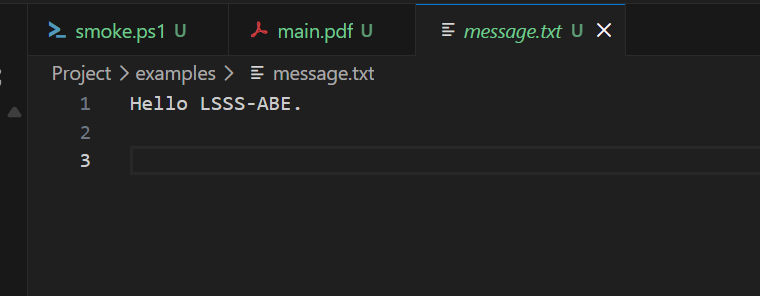
\includegraphics[width=0.72\textwidth]{examle_message.png}
\caption{原始明文 message.txt 截图}
\label{fig:screenshot-message-body}
\end{figure}

访问策略为：

\[
    (A\wedge B)\vee C.
\]

实验设计遵循两个原则。第一，测试场景必须覆盖访问结构的不同语义，包括 AND 分支、OR 分支、一般阈值门和不满足策略的情况。第二，测试不能只验证正常路径，还要覆盖工程边界，例如特殊属性名、密文篡改、重复属性和非法策略输入。这样可以为系统并非只对示例策略“刚好可用”提供实验依据，并展示其对常见边界输入的处理能力。

这些场景的选择与参考资料中的关键要求一一对应：Bethencourt 等人~[2]强调 CP-ABE 的访问策略由属性集合满足；Waters~[3]要求根据 $I=\{i:\rho(i)\in S\}$ 求重构常数；Liu 等人~[4]强调阈值访问树不应只局限于 AND/OR；实验三课件~[1]要求检验属性基加密算法实现是否正确。因此，测试既要有满足策略的成功样例，也必须有不满足策略、阈值门、重复属性和非法输入等反例或边界样例。

测试属性集合与边界检查设置如表 \ref{tab:test-scenarios} 所示。基础指数版包含九个场景；真实 pairing 版复用其中的核心语义，并在 BLS12-381 群元素上重新验证成功解密、拒绝解密、特殊属性名、密文篡改、一般阈值门、重复属性和非法策略输入。

\begin{table}[H]
\centering
\caption{测试场景设置}
\label{tab:test-scenarios}
\begin{tabular}{>{\raggedright\arraybackslash}p{0.10\textwidth} >{\raggedright\arraybackslash}p{0.25\textwidth} >{\raggedright\arraybackslash}p{0.29\textwidth} >{\raggedright\arraybackslash}p{0.20\textwidth}}
\toprule
场景 & 输入或操作 & 策略或对象 & 实验现象 \\
\midrule
1 & $\{A,B\}$ & $(A\wedge B)\vee C$ & 解密成功 \\
2 & $\{C\}$ & $(A\wedge B)\vee C$ & 解密成功 \\
3 & $\{A\}$ & $(A\wedge B)\vee C$ & 解密失败 \\
4 & \verb|role:admin| & 单属性策略 & 安全生成文件并解密成功 \\
5 & 篡改 \verb|payload.tag| & 密文 JSON & HMAC 拒绝 \\
6 & $\{D,F\}$ & $2$-of-$3(D,E,F)$ & 解密成功 \\
7 & $\{D\}$ & $2$-of-$3(D,E,F)$ & 解密失败 \\
8 & $\{X\}$ & 重复属性策略 $X\wedge X$ & 解密成功 \\
9 & \verb|k=0|、\verb|k>n|、缺失字段、空属性等 & 非法策略输入 & 加密前拒绝 \\
\bottomrule
\end{tabular}
\end{table}

\section{实验流程}

完整实验流程包括以下环节：

\begin{enumerate}
    \item 运行 Setup，生成公共参数和主密钥。
    \item 分别为 $\{A,B\}$、$\{C\}$、$\{A\}$ 生成用户私钥。
    \item 使用公共参数和访问策略加密示例明文。
    \item 使用 $\{A,B\}$ 和 $\{C\}$ 私钥解密，并与原始明文进行比对。
    \item 使用 $\{A\}$ 私钥尝试解密，记录不满足策略时的拒绝行为。
    \item 使用 \verb|role:admin| 验证属性名包含冒号时仍能生成安全私钥文件并解密。
    \item 篡改密文中的 \verb|payload.tag|，验证 HMAC 完整性检查会拒绝密文。
    \item 使用 $2$-of-$3$ 阈值策略验证一般阈值门的成功和失败路径。
    \item 使用重复属性策略验证多行映射到同一属性时的重构行为。
    \item 使用非法策略验证输入校验能在加密前拒绝错误访问树。
\end{enumerate}

上述流程在实验中由烟雾测试脚本统一执行。基础指数版脚本使用 \path{tests/artifacts} 目录重新生成密钥、密文和输出文件；真实 pairing 版脚本使用独立的 \path{tests/artifacts_pairing} 目录保存测试产物。这样可以保证两条路线的测试结果均来自各自完整流程，也避免指数版产物与 pairing 版产物混用。相比零散命令输出，完整的 smoke 输出更能反映项目整体复现情况。

烟雾测试脚本命令如下：

\begin{lstlisting}[language=bash,caption={烟雾测试命令}]
Set-Location .\Project
powershell -NoProfile -ExecutionPolicy Bypass -File .\tests\smoke.ps1
\end{lstlisting}

真实 pairing 路线使用独立脚本验证。该脚本调用同一个 PowerShell CLI，但增加 \verb|-Adapter| \verb|pairing| 参数，使命令转发到 Python BLS12-381 后端：

\begin{lstlisting}[language=bash,caption={真实 pairing 版烟雾测试命令}]
Set-Location .\Project
powershell -NoProfile -ExecutionPolicy Bypass -File .\tests\smoke_pairing.ps1
\end{lstlisting}

基础指数版关键输出如下：

\begin{lstlisting}[caption={基础指数版烟雾测试关键输出}]
Scenario 1 OK: {A,B} decrypted successfully.
Scenario 2 OK: {C} decrypted successfully.
Scenario 3 OK: {A} correctly rejected.
Scenario 4 OK: filename-safe attribute key for role:admin decrypted successfully.
Scenario 5 OK: tampered ciphertext correctly rejected.
Scenario 6 OK: {D,F} satisfied 2-of-3 threshold policy.
Scenario 7 OK: {D} correctly rejected by 2-of-3 threshold policy.
Scenario 8 OK: repeated attribute rows decrypted successfully.
Scenario 9 OK: invalid policies correctly rejected.
All smoke tests passed.
\end{lstlisting}

真实 pairing 版关键输出如下：

\begin{lstlisting}[caption={真实 pairing 版烟雾测试关键输出}]
Pairing scenario 1 OK: {A,B} decrypted successfully.
Pairing scenario 2 OK: {C} decrypted successfully.
Pairing scenario 3 OK: {A} correctly rejected.
Pairing scenario 4 OK: role:admin decrypted successfully.
Pairing scenario 5 OK: tampered ciphertext correctly rejected.
Pairing scenario 6 OK: 2-of-3 threshold behavior is correct.
Pairing scenario 7 OK: repeated attribute rows decrypted successfully.
Pairing scenario 8 OK: invalid policies correctly rejected.
All pairing smoke tests passed.
\end{lstlisting}

图 \ref{fig:screenshot-smoke-body} 展示了基础指数版真实终端中的烟雾测试完整输出，截图包含九个 OK 场景和最终通过提示。图 \ref{fig:screenshot-pairing-smoke-body} 展示了真实 pairing 路线的完整终端输出，截图中包含 conda 环境激活、进入项目源码目录、八类 pairing 场景和最终通过提示。两张截图分别对应指数抽象路线和 BLS12-381 真实配对路线，说明同一访问结构在两种底层群运算实现下均完成了成功解密、拒绝解密和边界输入验证。

\begin{figure}[H]
\centering
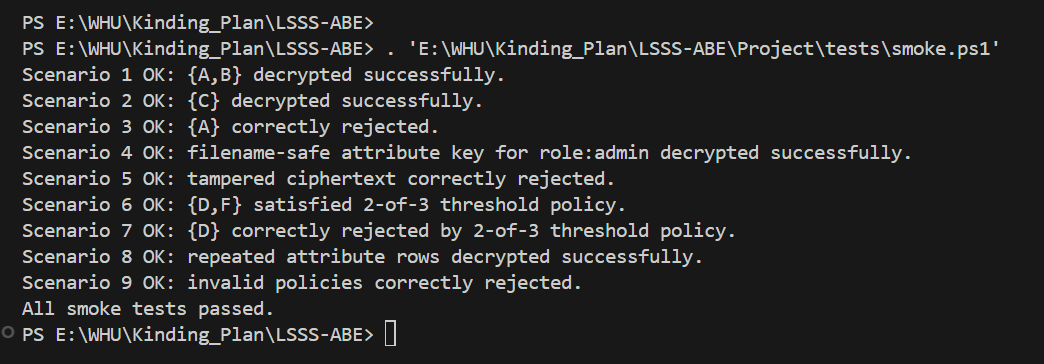
\includegraphics[width=0.92\textwidth]{All_Smoke_Tests_Pass.png}
\caption{基础指数版烟雾测试完整输出截图}
\label{fig:screenshot-smoke-body}
\end{figure}

\begin{figure}[H]
\centering
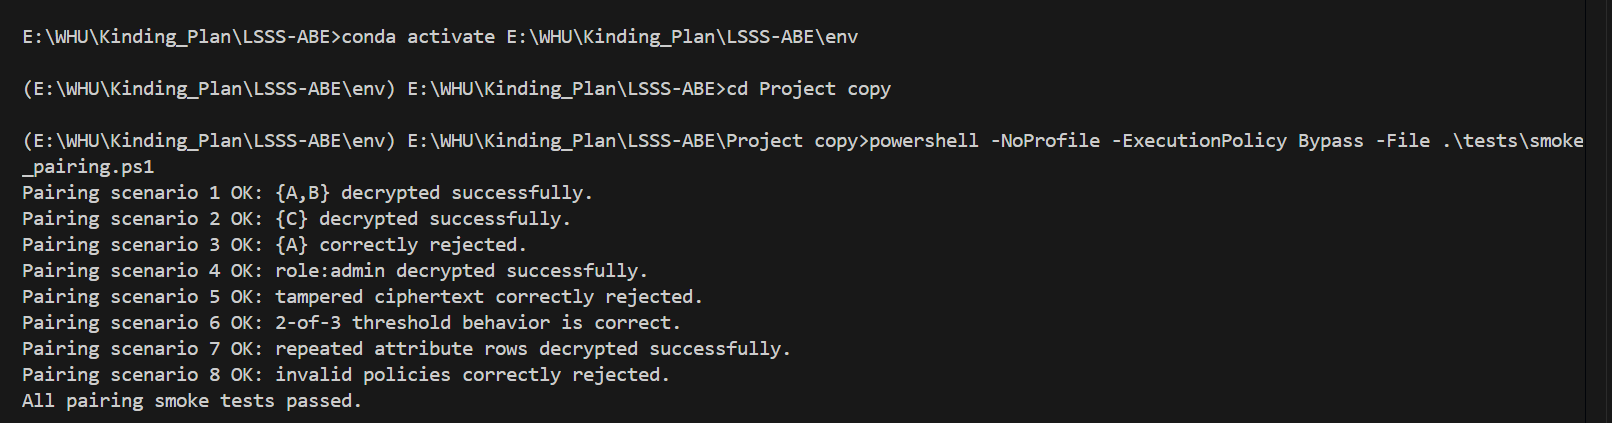
\includegraphics[width=0.95\textwidth]{pairing_smoke_tests_pass.png}
\caption{真实 pairing 路线烟雾测试完整输出截图}
\label{fig:screenshot-pairing-smoke-body}
\end{figure}

除统一烟雾测试外，本实验也保留了逐条运行 Setup、KeyGen、Encrypt 和 Decrypt 命令的结果。图 \ref{fig:screenshot-setup-body} 至图 \ref{fig:screenshot-decrypt-body} 展示了四个核心命令的实际运行截图。

\begin{figure}[H]
\centering
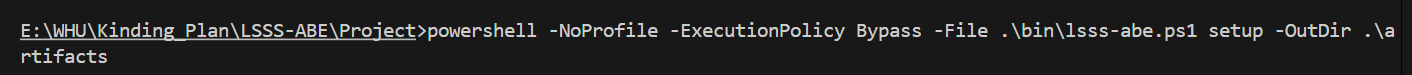
\includegraphics[width=0.95\textwidth]{setup.png}
\caption{Setup 命令运行截图}
\label{fig:screenshot-setup-body}
\end{figure}

\begin{figure}[H]
\centering
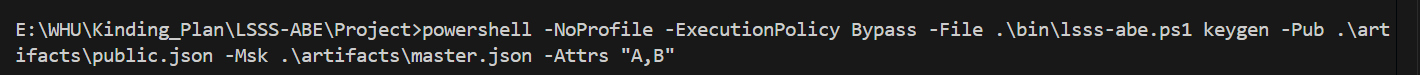
\includegraphics[width=0.95\textwidth]{keygen.png}
\caption{KeyGen 命令运行截图}
\label{fig:screenshot-keygen-body}
\end{figure}

\begin{figure}[H]
\centering
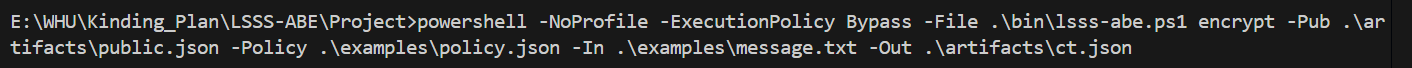
\includegraphics[width=0.95\textwidth]{encrypt.png}
\caption{Encrypt 命令运行截图}
\label{fig:screenshot-encrypt-body}
\end{figure}

\begin{figure}[H]
\centering
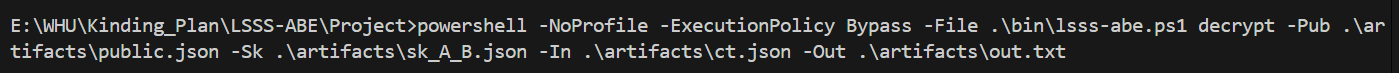
\includegraphics[width=0.95\textwidth]{decrypt.png}
\caption{Decrypt 命令运行截图}
\label{fig:screenshot-decrypt-body}
\end{figure}

这些输出行不仅是程序提示，也对应了后续结果分析中的每个检查点。场景一、二证明满足策略时能够恢复明文；场景三、七证明不满足策略时会被拒绝；场景五证明密文完整性检查生效；场景八和九则说明新增的边界行为已经被纳入自动化测试。

真实 pairing 输出的意义在于：同一访问策略和测试集合不再只通过指数抽象模型验证，而是已经在 BLS12-381 的 $G_1/G_2/G_T$ 群元素、真实配对、哈希到群和 $G_T$ 密钥派生路径下完成闭环。由于 pairing 版密钥和密文保存真实群元素编码，输出结果同时说明 Python 后端与 PowerShell CLI 的参数转发、JSON 文件读写和错误传播能够协同工作。

\section{实验结果}

实验结果如图 \ref{fig:experiment-results} 所示。九个检查点覆盖基础策略正反例、特殊属性名、密文完整性、一般阈值门、重复属性和非法策略输入。

\begin{figure}[H]
\centering
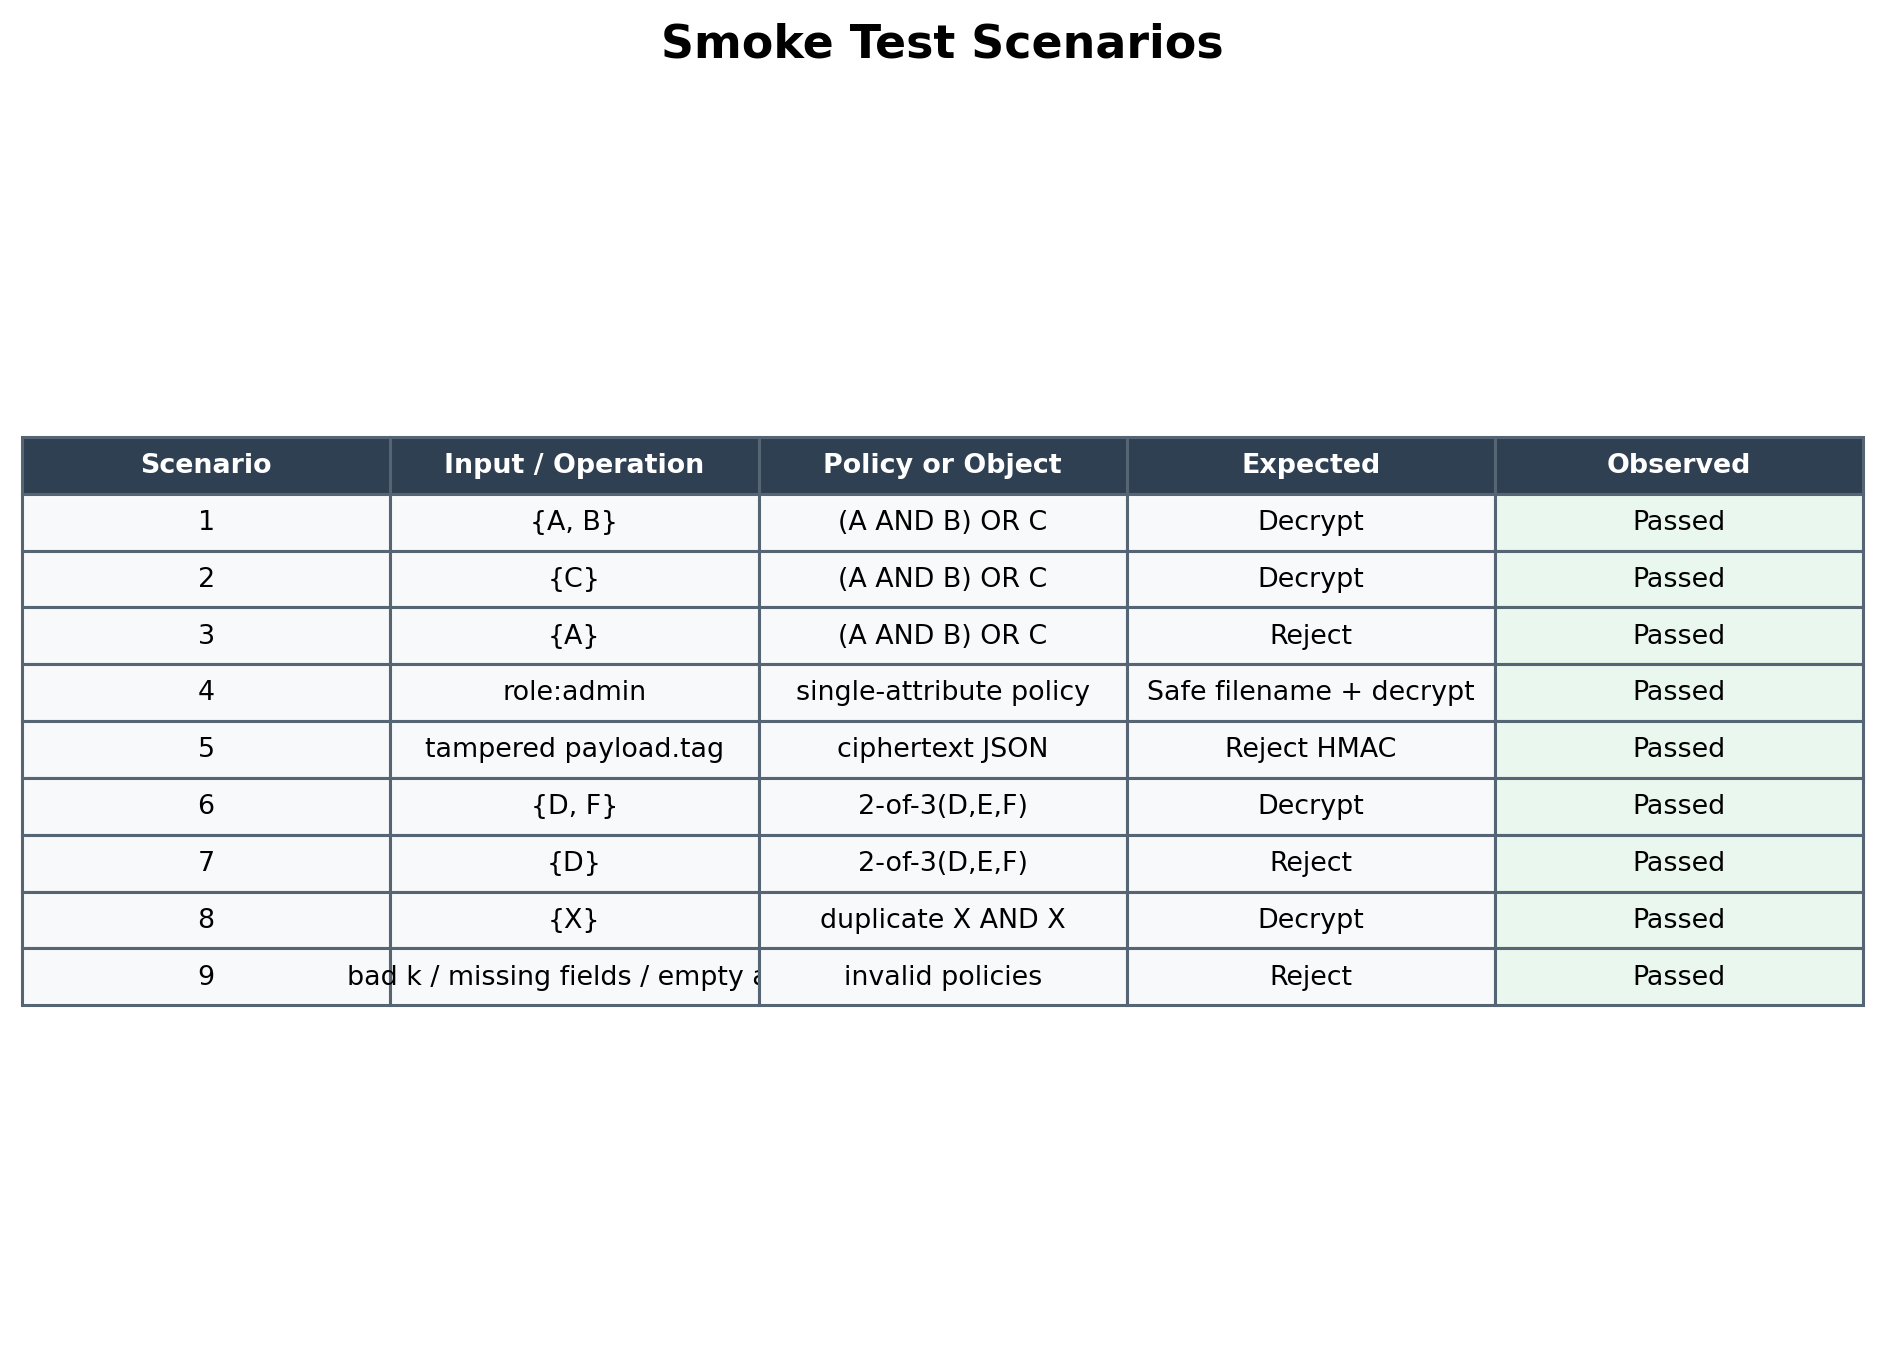
\includegraphics[width=0.90\textwidth]{experiment_results.png}
\caption{烟雾测试场景与结果}
\label{fig:experiment-results}
\end{figure}

\subsection[场景一：属性集合 AB]{场景一：属性集合 $\{A,B\}$}

当用户拥有 A 和 B 两个属性时，用户满足策略中的 AND 分支。矩阵中 A、B 两行分别为：

\[
    M_A=(1,1),\quad M_B=(1,2).
\]

求解重构系数可得：

\[
    2M_A-M_B=2(1,1)-(1,2)=(1,0).
\]

因此 $\{A,B\}$ 可以重构秘密 $s$，进而恢复消息指数 $m$，最终解出明文。实验输出文件 \verb|out_A_B.txt| 与原始 \verb|message.txt| 完全一致。

图 \ref{fig:screenshot-out-ab-body} 展示了使用属性集合 $\{A,B\}$ 解密后的输出文件。其内容与图 \ref{fig:screenshot-message-body} 中的原始明文一致。

\begin{figure}[H]
\centering
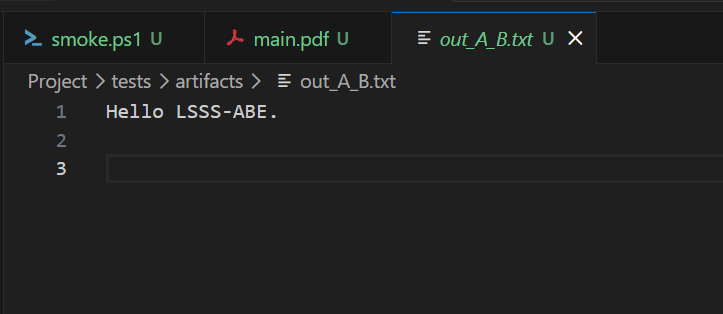
\includegraphics[width=0.72\textwidth]{tests_artifacts_out_A_B.png}
\caption{使用属性集合 \{A,B\} 解密后的输出截图}
\label{fig:screenshot-out-ab-body}
\end{figure}

这个场景验证的是最典型的 AND 分支。由于 A、B 两行都必须参与重构，缺少任意一行都不能得到 $(1,0)$。因此它不仅证明“满足策略可以解密”，也证明系统确实在使用 LSSS 线性组合，而不是简单检查某个单一属性。

\subsection[场景二：属性集合 C]{场景二：属性集合 $\{C\}$}

属性 C 对应矩阵行：

\[
    M_C=(1,0).
\]

该行本身已经等于重构目标 $(1,0)$，因此重构系数为 $1$，用户只凭属性 C 即可满足策略。实验输出文件 \verb|out_C.txt| 与原始明文一致。

图 \ref{fig:screenshot-out-c-body} 展示了使用属性集合 $\{C\}$ 解密后的输出文件。该截图说明 OR 分支对应的单行重构路径也能正确恢复明文。

\begin{figure}[H]
\centering
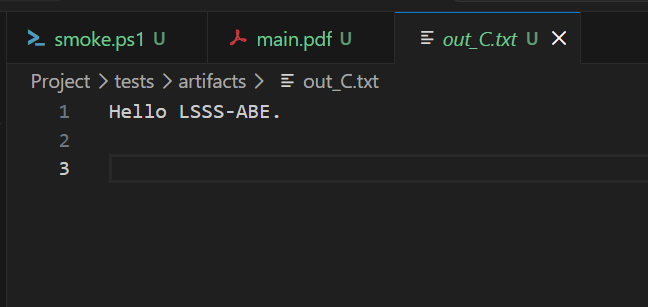
\includegraphics[width=0.72\textwidth]{tests_artifacts_out_C.png}
\caption{使用属性集合 \{C\} 解密后的输出截图}
\label{fig:screenshot-out-c-body}
\end{figure}

这个场景验证的是 OR 分支。与 $\{A,B\}$ 需要两行组合不同，属性 C 对应的行本身就可以恢复秘密。这说明同一个策略中可以同时存在“多属性共同满足”和“单属性直接满足”两种路径，系统能够由矩阵自然处理二者。

\subsection[场景三：属性集合 A]{场景三：属性集合 $\{A\}$}

如果用户只有属性 A，则可用矩阵只有：

\[
    M_A=(1,1).
\]

此时需要找到 $\omega$，使得：

\[
    \omega(1,1)=(1,0).
\]

该方程要求 $\omega=1$ 且 $\omega=0$ 同时成立，显然矛盾。因此线性方程无解，系统抛出：

\begin{lstlisting}[caption={不满足策略时的错误信息}]
Attributes do not satisfy policy.
\end{lstlisting}

图 \ref{fig:screenshot-sk-a-failed-body} 展示了使用 \verb|sk_A.json| 解密时的真实终端输出。截图中的核心错误信息为 ``Attributes do not satisfy policy.''，说明系统没有为不满足访问策略的属性集合输出明文。

\begin{figure}[H]
\centering
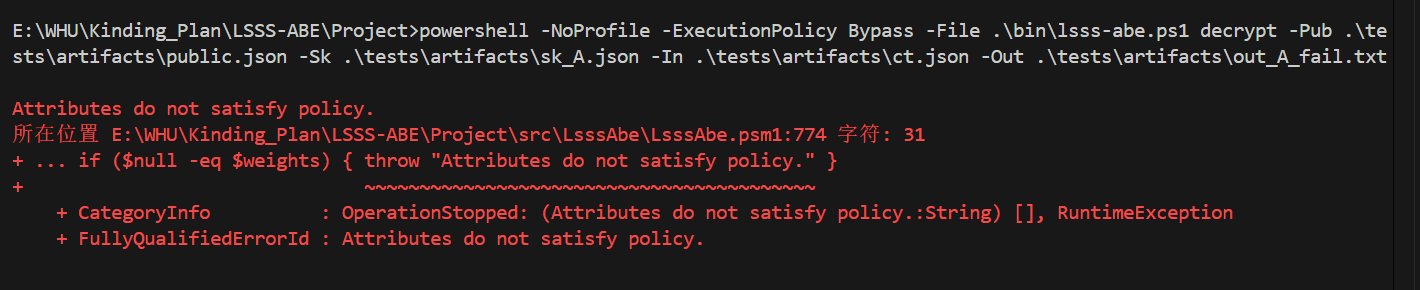
\includegraphics[width=0.95\textwidth]{sk_A_decrypt_failed.png}
\caption{使用 sk\_A.json 解密失败的终端截图}
\label{fig:screenshot-sk-a-failed-body}
\end{figure}

这说明系统不仅能验证成功路径，也能拒绝不满足策略的私钥。

失败场景在访问控制实验中非常重要。如果只有成功解密测试，无法排除系统“过度授权”的问题。$\{A\}$ 失败说明系统没有把 AND 分支错误地当作 OR 分支处理，也说明高斯消元能够识别无解方程组。

\subsection{场景四：特殊属性名 \texttt{role:admin}}

真实系统中的属性名往往不是单个字母，而可能是 \verb|role:admin|、\verb|dept:research| 等包含冒号的字符串。Windows 文件系统中冒号具有特殊含义，如果直接将属性名拼接为私钥文件名，可能产生非预期文件。当前 CLI 会先将属性名安全化，因此 \verb|role:admin| 对应输出文件为 \verb|sk_role_admin.json|，而私钥 JSON 内部仍保留原始属性名 \verb|role:admin|。测试结果表明，该属性既能安全生成文件，也能完成解密。

测试脚本中的演示代码如下。它首先构造单属性策略 \verb|role:admin|，随后检查私钥文件是否被安全命名为 \verb|sk_role_admin.json|，最后使用该私钥完成加解密。

\begin{lstlisting}[language=bash,caption={特殊属性名场景测试代码}]
[pscustomobject]@{ attr = "role:admin" } |
  ConvertTo-Json -Depth 10 |
  Set-Content -LiteralPath $specialPolicyPath -Encoding UTF8

& $bin keygen -Pub (Join-Path $art "public.json") `
  -Msk (Join-Path $art "master.json") `
  -OutDir $art -Attrs "role:admin"

$specialSkPath = Join-Path $art "sk_role_admin.json"
if (-not (Test-Path -LiteralPath $specialSkPath)) {
    throw "Scenario 4 failed: filename-safe secret key was not created."
}

& $bin encrypt -Pub (Join-Path $art "public.json") `
  -Policy $specialPolicyPath -In (Join-Path $root "examples\message.txt") `
  -Out $specialCtPath
& $bin decrypt -Pub (Join-Path $art "public.json") `
  -Sk $specialSkPath -In $specialCtPath -Out $specialOutPath
\end{lstlisting}

这个场景属于工程健壮性测试。真实属性名通常不会只由单个大写字母组成，可能包含部门、角色、等级等命名空间信息。文件名安全化如果处理不当，可能导致私钥文件无法生成，或者生成的文件名和属性语义不一致。该测试确认安全化只影响文件名，不影响策略匹配。

\subsection{场景五：密文篡改检测}

为验证对称载荷的完整性保护，测试脚本将已生成密文中的 \verb|payload.tag| 替换为错误 HMAC 标签，再尝试解密。系统在 AES 解密前重新计算 HMAC，并抛出：

\begin{lstlisting}[caption={密文篡改时的错误信息}]
Invalid ciphertext tag.
\end{lstlisting}

测试脚本中的核心做法是读取原始密文，替换认证标签字段，再尝试用满足策略的 A、B 私钥解密。由于 HMAC 校验失败，程序必须拒绝输出明文。

\begin{lstlisting}[language=bash,caption={密文篡改场景测试代码}]
$ctObj = Get-Content -Raw -LiteralPath (Join-Path $art "ct.json") `
  -Encoding UTF8 | ConvertFrom-Json
$ctObj.payload.tag = [Convert]::ToBase64String((New-Object byte[] 32))
$ctObj | ConvertTo-Json -Depth 100 |
  Set-Content -LiteralPath $tamperedCtPath -Encoding UTF8

try {
    & $bin decrypt -Pub (Join-Path $art "public.json") `
      -Sk (Join-Path $art "sk_A_B.json") `
      -In $tamperedCtPath -Out (Join-Path $art "out_tampered.txt")
    throw "Scenario 5 failed: tampered ciphertext should NOT decrypt."
} catch {
    if ($_.Exception.Message -notmatch "Invalid ciphertext tag") {
        throw "Scenario 5 failed: unexpected error."
    }
}
\end{lstlisting}

这说明密文载荷被篡改时不会被静默接受。

该测试也说明 CP-ABE 层和对称加密层之间的边界是清楚的。即使用户属性满足策略，如果密文载荷的认证标签错误，系统仍会拒绝输出明文。这避免了“访问策略满足就忽略密文完整性”的错误实现。

\subsection{场景六与七：2-of-3 阈值门}

为验证访问控制树中一般阈值门的处理能力，测试脚本构造了 $2$-of-$3(D,E,F)$ 策略。属性集合 $\{D,F\}$ 满足该策略，因此可以解密；属性集合 $\{D\}$ 只包含一个属性，不满足 $2$-of-$3$ 条件，因此被拒绝。这一测试表明，系统并非只支持 AND/OR 特例，也能处理一般阈值门。

测试脚本中的关键代码如下。前半部分构造阈值策略并验证 $\{D,F\}$ 成功；后半部分只为属性 D 生成私钥，并要求系统拒绝解密。

\begin{lstlisting}[language=bash,caption={2-of-3 阈值门成功与失败测试代码}]
[pscustomobject]@{
    k = 2
    children = @(
        [pscustomobject]@{ attr = "D" },
        [pscustomobject]@{ attr = "E" },
        [pscustomobject]@{ attr = "F" }
    )
} | ConvertTo-Json -Depth 10 |
  Set-Content -LiteralPath $thresholdPolicyPath -Encoding UTF8

& $bin keygen -Pub (Join-Path $art "public.json") `
  -Msk (Join-Path $art "master.json") -OutDir $art -Attrs "D,F"
& $bin encrypt -Pub (Join-Path $art "public.json") `
  -Policy $thresholdPolicyPath -In (Join-Path $root "examples\message.txt") `
  -Out $thresholdCtPath
& $bin decrypt -Pub (Join-Path $art "public.json") `
  -Sk (Join-Path $art "sk_D_F.json") `
  -In $thresholdCtPath -Out $thresholdOutPath

& $bin keygen -Pub (Join-Path $art "public.json") `
  -Msk (Join-Path $art "master.json") -OutDir $art -Attrs "D"
try {
    & $bin decrypt -Pub (Join-Path $art "public.json") `
      -Sk (Join-Path $art "sk_D.json") `
      -In $thresholdCtPath -Out (Join-Path $art "out_D.txt")
    throw "Scenario 7 failed: {D} should NOT satisfy 2-of-3 policy."
} catch {
    if ($_.Exception.Message -notmatch "Attributes do not satisfy") {
        throw "Scenario 7 failed: unexpected error."
    }
}
\end{lstlisting}

这两个场景扩展了示例策略的覆盖范围。AND 和 OR 都可以看成阈值门的特例，但如果不单独测试 $2$-of-$3$，仍难以说明实现已经覆盖一般阈值门路径。通过同时测试 $\{D,F\}$ 成功和 $\{D\}$ 失败，可以确认阈值条件不是被简单地写死为“至少一个”或“全部”。

\subsection{场景八：重复属性}

重复属性测试构造策略 $X\wedge X$，其 LSSS 矩阵中会出现多行映射到同一属性 X。解密端筛选行时会把所有 $\rho(i)=X$ 的行都纳入线性方程求解，并复用私钥中的同一个 $K_X$ 分量完成计算。该测试用于验证系统能够处理“多行映射到同一属性”的工程场景。

测试脚本中的核心代码如下。它先构造两个叶子均为 X 的 $2$-of-$2$ 策略，再只为属性 X 生成私钥；如果系统没有正确处理重复属性行，该场景会在解密或明文比对阶段失败。

\begin{lstlisting}[language=bash,caption={重复属性场景测试代码}]
[pscustomobject]@{
    k = 2
    children = @(
        [pscustomobject]@{ attr = "X" },
        [pscustomobject]@{ attr = "X" }
    )
} | ConvertTo-Json -Depth 10 | Set-Content -LiteralPath $duplicatePolicyPath -Encoding UTF8

& $bin keygen -Pub (Join-Path $art "public.json") -Msk (Join-Path $art "master.json") -OutDir $art -Attrs "X"
& $bin encrypt -Pub (Join-Path $art "public.json") -Policy $duplicatePolicyPath -In (Join-Path $root "examples\message.txt") -Out $duplicateCtPath
& $bin decrypt -Pub (Join-Path $art "public.json") -Sk (Join-Path $art "sk_X.json") -In $duplicateCtPath -Out $duplicateOutPath

$outDuplicate = Get-Content -Raw -LiteralPath $duplicateOutPath -Encoding UTF8
if ($orig -ne $outDuplicate) {
    throw "Scenario 8 failed: repeated attribute rows should decrypt with attribute X."
}
\end{lstlisting}

\subsection{场景九：非法策略输入}

非法策略测试包含多类错误访问树：阈值 $k=0$、$k$ 大于子节点数量、缺失 $k$、子节点列表为空、属性名为空，以及叶子节点同时携带 \verb|children|。系统在树到 LSSS 矩阵转换前执行递归校验，并在发现非法结构时抛出 \verb|Invalid policy| 相关错误。这样可以避免非法访问树进入矩阵构造流程，减少后续难以定位的运行时异常。

非法策略测试不是只检查单个错误输入，而是把多类错误访问树组织成数组逐个加密。实验现象是每个非法策略都在加密阶段抛出 \verb|Invalid policy| 相关错误，且没有任何非法策略生成可用密文。

\begin{lstlisting}[language=bash,caption={非法策略输入场景测试代码}]
$invalidPolicies = @(
    [pscustomobject]@{ Name = "k0"; Policy = [pscustomobject]@{ k = 0; children = @([pscustomobject]@{ attr = "Z" }) } },
    [pscustomobject]@{ Name = "k_too_large"; Policy = [pscustomobject]@{ k = 3; children = @([pscustomobject]@{ attr = "Y" }, [pscustomobject]@{ attr = "Z" }) } },
    [pscustomobject]@{ Name = "missing_k"; Policy = [pscustomobject]@{ children = @([pscustomobject]@{ attr = "Z" }) } },
    [pscustomobject]@{ Name = "empty_children"; Policy = [pscustomobject]@{ k = 1; children = @() } },
    [pscustomobject]@{ Name = "empty_attr"; Policy = [pscustomobject]@{ attr = "" } },
    [pscustomobject]@{ Name = "leaf_with_children"; Policy = [pscustomobject]@{ attr = "Q"; children = @([pscustomobject]@{ attr = "R" }) } }
)

$invalidPoliciesRejected = 0
foreach ($case in $invalidPolicies) {
    $invalidPolicyPath = Join-Path $art "policy_invalid_$($case.Name).json"
    $case.Policy | ConvertTo-Json -Depth 10 | Set-Content -LiteralPath $invalidPolicyPath -Encoding UTF8
    try {
        & $bin encrypt -Pub (Join-Path $art "public.json") -Policy $invalidPolicyPath -In (Join-Path $root "examples\message.txt") -Out (Join-Path $art "ct_invalid.json")
        throw "Invalid policy should not encrypt: $invalidPolicyPath"
    } catch {
        if ($_.Exception.Message -notmatch "Invalid policy") {
            throw "Scenario 9 failed: unexpected error for invalid policy."
        }
        $invalidPoliciesRejected++
    }
}
\end{lstlisting}

通过把非法策略统一放入数组，测试脚本保留了继续扩展的空间，例如非整数 \verb|k|、空根节点、缺失 \verb|children| 或更复杂的畸形 JSON。当前实现已经覆盖了最容易导致矩阵构造错误的几类输入，因此能更早暴露策略格式问题。

\section{结果分析}

从实验现象看，九个场景形成了一条较完整的证据链。场景一和场景二分别对应示例策略 $(A\wedge B)\vee C$ 的 AND 分支和 OR 分支，二者都能恢复原始明文，说明系统生成的密钥分量、密文分量和对称载荷可以完成一次完整的加密解密闭环。场景三使用属性集合 $\{A\}$ 尝试解密并被拒绝，说明系统没有把 ``拥有部分属性'' 错误地视为满足策略。成功路径和失败路径同时成立，才能说明访问控制不是形式上的字符串比较，而是由矩阵重构条件决定。

从 LSSS 角度看，实验结果说明访问树语义与线性重构语义保持一致。加密阶段把访问树转换为矩阵 $(M,\rho)$，解密阶段根据用户属性集合 $S$ 选取行集合 $I=\{i:\rho(i)\in S\}$，再求解 $M_I^T\omega=e_1$。当属性集合为 $\{A,B\}$ 时，A 行和 B 行可以共同重构第一维；当属性集合为 $\{C\}$ 时，C 行单独即可完成重构；当属性集合为 $\{A\}$ 时，可用行不足以重构第一维，因此线性方程无解。由此可以看出，程序判断策略满足性时依赖的是 LSSS 的线性代数条件，而不是针对示例策略手写 AND/OR 判断分支。

一般阈值门测试进一步扩展了这一结论。$2$-of-$3(D,E,F)$ 场景中，$\{D,F\}$ 能够解密而 $\{D\}$ 被拒绝，说明系统处理的不是简单的 ``至少一个属性满足'' 或 ``全部属性满足'' 两种特例，而是按照阈值 $k$ 和子节点数 $n$ 共同决定访问条件。该结果与第三章中访问树一般性的设计相互对应：内部节点统一保存 $k$ 与 \verb|children|，矩阵构造阶段为阈值门引入 $k-1$ 个随机维度，解密阶段再由行集合可重构性给出最终判定。

工程边界测试说明实验对象不仅停留在理想公式输入上。特殊属性名 \verb|role:admin| 能够生成安全文件名并保留原始属性语义，说明 CLI 文件系统处理没有破坏策略匹配；密文篡改测试在 HMAC 检查阶段被拒绝，说明满足访问策略并不会绕过对称载荷完整性验证；重复属性 $X\wedge X$ 能够成功重构，说明 $\rho$ 允许多行映射到同一属性，解密端没有错误地只保留某个属性的第一行；非法策略输入在加密前被拒绝，说明策略校验可以在矩阵构造前截断明显错误的访问树结构。

从实验覆盖关系看，各场景可以归纳为四类。第一类是正确性场景，验证满足策略时明文能够被恢复；第二类是拒绝场景，验证不满足策略或密文被篡改时不会输出明文；第三类是表达能力场景，验证一般阈值门和重复属性行能够被 LSSS 机制处理；第四类是输入健壮性场景，验证特殊属性名和非法策略不会破坏系统运行。四类结果共同支撑本章结论：本项目实现的核心并非一次孤立的文件加密演示，而是围绕访问控制树、LSSS 矩阵、属性私钥和线性重构建立了可复现实验链路。

结合课程题目要求，这组实验能够说明系统已经完成两个主要目标：其一，访问控制树能够自动转换为 LSSS 矩阵，并在密文中以可检查形式保存；其二，Setup、KeyGen、Encrypt 和 Decrypt 四个算法能够围绕该矩阵形成完整流程，并区分满足策略与不满足策略的属性集合。与实验三课件~[1]中关于 Waters 2011 方案~[3]和 FABEO 方案~[5]的加解密测试要求相比，本项目的检验重点更集中在 LSSS-CP-ABE 的访问结构语义上。也就是说，本实验不只比较一次明文和解密输出是否相同，而是通过多种属性集合和边界场景验证矩阵重构条件与访问树语义的一致性。

需要说明的是，本章实验结论分为两个层次。指数抽象版验证了 LSSS-CP-ABE 的矩阵构造、份额重构和访问控制行为，便于解释公式中的代数抵消；真实 pairing 版进一步验证了同一访问结构可以在 BLS12-381 群元素和真实配对运算上运行，说明底层群运算真实化后核心链路仍然成立。二者仍不能被直接解释为完整安全证明，因为形式化安全还涉及所选论文模型、随机数采样、哈希到群、序列化检查、参数选择和攻击模型等条件。复杂嵌套阈值树、更多畸形 JSON 结构和更严格的密文结构校验仍属于后续可继续扩展的验证对象。

\chapter{总结与展望}

\section{工作总结}

本实验完成了一个基于 LSSS 矩阵的 CP-ABE 实验实现。系统以访问控制树作为策略输入，自动构造 LSSS 矩阵，并使用线性重构判断用户属性集合是否满足策略。围绕这一主线，项目实现了 Setup、KeyGen、Encrypt 和 Decrypt 四个核心流程，并通过命令行脚本和烟雾测试验证了成功解密和拒绝解密两类行为。同时，系统在同一 \verb|Project| 工程中接入了基于 \verb|py-ecc| 的 BLS12-381 真实 pairing 后端，使同一 LSSS-CP-ABE 主线能够在真实 $G_1/G_2/G_T$ 群元素和配对运算上运行。

从理论角度看，本实验把 CP-ABE 的访问控制问题转化为线性代数问题。访问树中的 AND、OR 和阈值门被统一表示为 LSSS 矩阵行，解密时不再依赖针对具体树结构的递归判定，而是求解 $M_I^T\omega=e_1$。这一设计有助于理解 Waters 类 CP-ABE 构造中“线性秘密共享”和“双线性对抵消”之间的关系。

这一结论与主要参考资料的脉络一致：Bethencourt 等人~[2]给出了 CP-ABE 的密文策略访问控制模型，Waters~[3]将表达能力推进到 LSSS 矩阵表示，Liu 等人~[4]进一步讨论如何从更直观的阈值访问树生成 LSSS 矩阵。本文的贡献不是提出新的密码方案，而是把这些资料中的核心机制整理成可运行、可检查、可复现的课程实验系统。

从工程角度看，项目使用 PowerShell 和 .NET 标准库完成基础实现，具有较低复现门槛。密钥、密文、策略和矩阵均以 JSON 形式保存，便于实验检查、调试和结果分析。真实 pairing 路线进一步通过 Python 后端调用真实配对库，在保持 CLI 使用方式基本一致的同时，把底层群元素从整数指数推进到 BLS12-381 曲线点和 $G_T$ 元素。对称加密部分采用 AES-CBC-HMAC 组合，体现了“先加密再认证”的基本工程思想。

在结果呈现上，本文将公式、代码和实验现象对应起来。例如，第二章解释 LSSS 重构条件，第三章说明加解密公式，第四章给出关键代码片段，第五章再用九个场景验证这些设计。这样的组织方式使算法实现、程序输出和访问策略语义保持一致。

\section{主要完成内容}

本项目已经完成的主要内容包括：

\begin{enumerate}
    \item 定义访问控制树 JSON 格式，支持属性叶子和阈值门。
    \item 实现访问控制树到 LSSS 矩阵的自动转换。
    \item 实现模 $p$ 下的大整数运算、向量运算、快速幂和模逆。
    \item 实现 LSSS 重构系数求解，使用高斯消元判断属性集合是否满足策略。
    \item 实现 CP-ABE 的 Setup、KeyGen、Encrypt 和 Decrypt 流程。
    \item 实现 BLS12-381 真实 pairing 后端，支持 $G_1/G_2/G_T$ 群元素、哈希到 $G_1$、配对运算、序列化和基本成员检查。
    \item 使用 AES-CBC-HMAC 加密和认证实际明文载荷。
    \item 编写 CLI 脚本，使各阶段可以独立运行和观察结果。
    \item 编写烟雾测试，验证基础正反例、特殊属性名、密文篡改、$2$-of-$3$ 阈值门、重复属性和非法策略输入，并对真实 pairing 路线进行补充验证。
    \item 编写 LaTeX 报告，解释理论基础、方案设计、系统实现和实验结果。
\end{enumerate}

这些完成内容覆盖了课程题目中的两个关键词：一是“属性基加密方案”，对应 Setup、KeyGen、Encrypt 和 Decrypt 四个流程；二是“使用访问控制树构建 LSSS 矩阵”，对应策略 JSON、矩阵转换函数和重构系数求解函数。烟雾测试中的阈值门、重复属性和非法策略输入进一步说明系统不是只针对一个固定样例硬编码。

\section{实验价值}

本实验的价值主要体现在三个方面。

第一，它将抽象的访问结构转化过程具体化。LSSS 在论文中常以矩阵形式出现，但矩阵如何由策略树生成并不直观。本项目通过示例策略 $(A\wedge B)\vee C$ 展示了从树到矩阵的完整过程，使矩阵行、属性映射和重构系数之间的关系更加清楚。

第二，它把 CP-ABE 的正确性验证拆解为可观察的中间步骤。密文中保留了策略、矩阵、行属性和指数分量，使每个字段在解密中的作用都能与算法公式对应起来。

第三，它提供了由浅入深的实验平台。指数抽象模型保留代数结构，使课程重点集中在访问策略、秘密共享和算法流程上；真实 pairing 路线则把同一主线放入 BLS12-381 群元素和配对运算中运行，使实验从“公式结构可解释”进一步推进到“真实群运算可执行”。

除此之外，项目还具有一定的可扩展价值。由于策略解析、矩阵构造、重构求解和 CP-ABE 主流程之间的边界较清晰，真实 pairing 接入时主要替换对象是群运算和序列化层，访问树到 LSSS 的构造逻辑仍可保留。真实 pairing 接入结果说明，先建立指数抽象模型再替换底层群实现是一条可行的工程路线。

Riepel 和 Wee 的 FABEO 方案~[5]表明，真实 ABE 研究还会继续优化配对次数、密钥和密文大小，并讨论自适应安全和多密文安全等更强性质。与这些研究方向相比，本项目已经完成课程题目所要求的 LSSS-ABE 主线，但距离高性能、可部署的 ABE 系统仍有明显距离。

\section{不足与限制}

本项目仍存在明显限制，主要包括：

\begin{itemize}
    \item \textbf{安全证明仍未形式化完成。} 真实 pairing 路线已经使用 BLS12-381 真实群元素和配对运算，但还没有逐条证明其与 Waters 2011 安全模型完全一致。
    \item \textbf{指数抽象版仍只适合解释代数结构。} 该路线没有真实双线性群中的困难问题保证，主要用于快速复现和公式对应。
    \item \textbf{参数与库选择仍需进一步论证。} BLS12-381 后端提升了实现真实性，但正式安全声明仍需要说明曲线选择、哈希到群域分离、随机数采样和库版本假设。
    \item \textbf{策略输入形式较基础。} 当前需要手写 JSON 访问树，尚未支持自然布尔表达式解析。
    \item \textbf{输入校验仍有扩展空间。} 当前已能拒绝非法阈值策略和空属性，但对密文数组长度不一致等异常结构的检查还可以进一步细化。
    \item \textbf{测试覆盖仍有扩展空间。} 当前指数版与 pairing 版烟雾测试已覆盖核心正反例、一般阈值门、特殊属性名、密文篡改、重复属性和非法策略输入；复杂嵌套策略、畸形 JSON 和文件覆盖行为仍属于可继续补充的测试维度。
    \item \textbf{CLI 输出仍有扩展空间。} 当前已对属性名生成文件名时做安全化处理，但输出路径、错误信息和运行状态提示仍可以进一步规范。
\end{itemize}

这些限制构成本文安全性声明的边界。指数抽象模型能够说明公式结构和访问控制逻辑正确，但不覆盖真实部署环境中的困难问题假设；真实 pairing 路线已经覆盖真实群元素和配对调用，但仍需要更严格的安全模型对齐和实现级审查。对课程实验而言，这种边界说明表明项目区分了算法流程验证、真实群运算实现和形式化安全证明三个层次。

\section{真实安全证明条件对照}

为了进一步说明指数模型、真实 pairing 实现与论文安全证明之间的关系，表 \ref{tab:security-proof-conditions} 给出安全证明条件对照。这里以 Waters 2011 风格的 LSSS-CP-ABE 构造~[3]为主要参照，关注实现是否满足论文安全模型的前提。

\begingroup
\renewcommand{\arraystretch}{1.18}
\begin{longtable}{>{\raggedright\arraybackslash}p{0.18\textwidth} >{\raggedright\arraybackslash}p{0.74\textwidth}}
\caption{安全证明条件对照}
\label{tab:security-proof-conditions}\\
\toprule
条件 & 对照说明 \\
\midrule
\endfirsthead
\toprule
条件 & 对照说明 \\
\midrule
\endhead
\textbf{双线性群} &
\textbf{真实实现：}使用素数阶配对友好曲线，提供 $G_1,G_2,G_T$ 和非退化双线性映射 $e:G_1\times G_2\rightarrow G_T$。\newline
\textbf{当前状态：}指数抽象路线使用 \texttt{ExponentSimulation}；真实 pairing 路线使用 \texttt{py-ecc} 的 BLS12-381 $G_1/G_2/G_T$ 与 \texttt{pairing}，已具备真实配对运算基础。\\[0.45em]
\textbf{群运算接口} &
\textbf{真实实现：}群元素乘法、幂运算、逆元、配对运算和目标群运算均由真实密码库实现。\newline
\textbf{当前状态：}\texttt{-Adapter pairing} 路线已由 Python 后端实现真实群元素计算；指数路线继续保留为解释和对照实现。\\[0.45em]
\textbf{随机数生成} &
\textbf{真实实现：}所有 $\mathbb{Z}_p$ 标量必须由密码学安全随机源均匀采样。\newline
\textbf{当前状态：}指数版使用 .NET 随机数生成器；pairing 版使用 Python \texttt{secrets.randbelow} 在曲线阶内采样。正式安全声明仍需进一步论证采样和参数选择。\\[0.45em]
\textbf{属性映射} &
\textbf{真实实现：}属性应按论文要求映射到群元素或公共参数；若使用哈希到群，应采用标准哈希到曲线方法。\newline
\textbf{当前状态：}指数版把属性哈希为标量；pairing 版调用 \texttt{hash\_to\_G1}，并使用固定 DST 将属性字符串映射为 $G_1$ 点。\\[0.45em]
\textbf{序列化检查} &
\textbf{真实实现：}反序列化群元素时必须检查编码合法性、曲线成员关系、子群成员关系和无穷远点。\newline
\textbf{当前状态：}pairing 版 JSON 保存 $G_1/G_2$ 坐标和 $G_T$ 系数，并在反序列化时检查曲线成员关系和子群成员关系；仍可继续增强无穷远点拒绝策略和异常密文测试。\\[0.45em]
\textbf{算法一致性} &
\textbf{真实实现：}Setup、KeyGen、Encrypt、Decrypt 的群元素位置、指数关系和访问结构必须与选定论文方案一致。\newline
\textbf{当前状态：}四算法结构与本文采用的 LSSS-CP-ABE 实验公式一致；pairing 版已经将 $K,L,K_x,C,C_0,C_i,D_i$ 分别落到 $G_1/G_2/G_T$ 对应位置。\\[0.45em]
\textbf{安全声明范围} &
\textbf{真实实现：}只能声明与论文模型相匹配的安全性，例如选择安全或自适应安全，并说明 CPA/CCA 范围。\newline
\textbf{当前状态：}实验结论限定为 LSSS-CP-ABE 的代数正确性、访问控制语义和真实 pairing 路径可运行性；不扩展为完整真实部署安全性。\\
\bottomrule
\end{longtable}
\endgroup

基于上述对照，可以得到一个更准确的结论：当前项目已经从单纯指数抽象验证推进到真实 BLS12-381 pairing 初步实现，验证了 LSSS-CP-ABE 的代数正确性、访问控制语义和真实群运算路径可运行性；若要进一步满足论文级安全证明条件，还需要将 Setup、KeyGen、Encrypt、Decrypt、哈希到群、随机数生成、序列化检查和安全声明逐项与选定论文的安全模型严格对齐。

\section{后续工作展望}

当前实现已经覆盖课程题目要求的 LSSS-ABE 主线，并在同一 \verb|Project| 工程中完成真实 pairing 初步接入。后续工作的核心不是重新设计访问控制树或 LSSS 矩阵构造，而是在保持现有模块边界的基础上，把真实 pairing 实现的安全模型对齐、策略表达能力、测试覆盖范围和实验呈现一致性进一步推进。四个方向之间也存在依赖关系：真实配对后端决定系统能否进入更接近真实密码实现的层面，策略语言和输入校验决定外部策略表达的可靠性，测试集决定边界行为是否稳定，实验呈现则负责把这些变化反映到报告证据链中。

\subsection{完善真实双线性对库实现}

真实 pairing 路线已经使用 \verb|py-ecc| 接入 BLS12-381，提供 $G_1$、$G_2$、$G_T$、$\mathbb{Z}_p$ 和配对映射 $e:G_1\times G_2\rightarrow G_T$。这一步使系统不再只停留在整数指数模拟层面，而是能够生成真实曲线点、调用真实配对函数，并把 $G_T$ 元素用于会话密钥派生。后续完善的重点，是把这一可运行实现继续向论文安全模型和工程健壮性靠拢。

现有结果说明群运算适配器边界是有效的。访问树解析、LSSS 矩阵生成和重构系数求解都只依赖标量和矩阵，不依赖具体群元素编码；因此真实化过程中稳定性较高的部分是策略层和线性代数层，变化最大的部分是 Setup、KeyGen、Encrypt、Decrypt 中的群元素表示、序列化格式和配对计算。换言之，当前实现已经把“访问结构正确性”和“底层群实现真实性”分开，这使系统能够同时保留指数抽象版和真实 pairing 版。

真实 pairing 版仍有进一步加固空间。群元素反序列化已经检查曲线成员关系和子群成员关系，但还可以加入更细的无穷远点拒绝、字段范围检查和异常密文测试；属性哈希已经使用 \verb|hash_to_G1|，但仍需在报告中固定域分离标签和哈希套件说明；随机标量采样已经使用安全随机源，但正式安全声明仍需说明采样均匀性；对称密钥派生则需要明确 $G_T$ 元素编码到固定长度密钥的规范。这些问题不属于 LSSS 矩阵转换本身，却直接影响真实 CP-ABE 实现能否更严谨地满足论文安全模型。

以实验三课件~[1]和 Waters 2011 方案~[3]为参照，真实化版本的比较对象还包括 FABEO 方案~[5]。Waters 方案更适合验证 LSSS 矩阵和重构常数进入加解密公式的方式，FABEO 方案则体现了较新 ABE 研究对密文大小、私钥大小、配对次数和安全模型的进一步优化。这样的对比能够把本实验从单一实验原型推进到不同 CP-ABE 构造之间的结构比较。

\subsection{增强策略语言}

当前系统使用 JSON 访问树作为策略输入，内部结构清晰，适合程序直接读取和递归校验；不足之处在于策略书写形式较接近中间表示，不够接近自然权限表达。策略语言扩展的目标，是在 JSON 访问树之前增加一层布尔表达式解析，外部输入形式例如：

\[
    (A \text{ AND } B) \text{ OR } C.
\]

解析层的输出仍然是当前系统已经支持的访问树结构。由此形成外部语法和内部表示的解耦：外部语法面向策略书写，内部 JSON 面向矩阵构造。AND、OR 和阈值门仍然统一归约为 $k$-of-$n$ 节点，后续 LSSS 转换函数无需改变。对于 \verb|role:admin|、\verb|dept:research| 这类带命名空间的属性，解析器还承担区分属性名冒号与语法操作符的任务，避免把合法属性名误判为非法表达式。

策略语言增强也与输入校验相关。表达式解析阶段能够发现括号不匹配、连续操作符、空属性、未知门类型等语法错误；访问树校验阶段则继续负责检查阈值 $k$、子节点数量和叶子节点结构。两级校验分别对应“外部策略文本是否合法”和“内部访问树是否能生成 LSSS 矩阵”，使错误来源更加明确。

\subsection{扩展测试集}

现有烟雾测试已经覆盖基础正反例、特殊属性名、密文篡改、一般阈值门、重复属性和非法策略输入。进一步扩展测试集时，重点在于增加策略结构深度、失败路径种类和异常密文形态，使测试不只覆盖示例策略，也覆盖更复杂的 LSSS 构造情形。

\begin{table}[H]
\centering
\caption{后续测试覆盖维度}
\begin{tabular}{>{\raggedright\arraybackslash}p{0.22\textwidth} >{\raggedright\arraybackslash}p{0.32\textwidth} >{\raggedright\arraybackslash}p{0.34\textwidth}}
\toprule
测试维度 & 代表场景 & 分析价值 \\
\midrule
嵌套策略 & 多层 AND/OR/阈值门组合 & 验证递归份额传播和随机列分配是否稳定。\\
失败路径 & 只满足局部子树但不满足根节点 & 验证线性重构不会把局部满足误判为全局满足。\\
异常密文 & 缺失 \verb|Ci|、\verb|Di| 或数组长度不一致 & 验证解密阶段对密文字段结构的检查能力。\\
策略语法 & 畸形 JSON、非法阈值、空属性、重复属性 & 验证策略校验能在矩阵构造前截断错误输入。\\
文件行为 & 输出路径已存在、属性名含特殊字符 & 验证 CLI 层对工程边界的处理稳定性。\\
\bottomrule
\end{tabular}
\end{table}

这些测试维度分别覆盖算法正确性和工程健壮性。嵌套策略和失败路径更接近 LSSS 理论层面，能够暴露矩阵列数、行映射和重构系数求解中的问题；异常密文、策略语法和文件行为更接近工程层面，能够暴露 JSON 结构、路径处理和错误信息中的问题。二者结合后，测试结果才能较充分地支撑“系统不仅能跑通示例，也能处理边界情况”的结论。

\subsection{实验呈现的一致性}

本报告的实验呈现围绕“理论定义、程序实现、文件结果和运行现象”之间的对应关系展开。系统架构图用于说明模块边界，加解密数据流图用于说明四个核心算法之间的数据传递，策略到 LSSS 矩阵的转换图用于说明访问树如何进入线性秘密共享结构；关键代码节选、密文 JSON 字段、烟雾测试输出和真实终端截图则分别对应实现依据、文件证据和运行结果。由此，报告中的图、表、代码和截图不是相互独立的材料，而是共同指向同一条实验链路。

这种呈现方式使第五章的实验结果能够被追溯到前文的算法设计。成功解密场景不仅有终端输出，也能对应到访问策略、LSSS 行集合和重构方程；失败解密场景不仅表现为错误信息，也能对应到属性集合无法满足 $M_I^T\omega=e_1$ 的线性条件；密文篡改、重复属性和非法策略输入等边界场景，则分别对应对称载荷完整性、行属性映射 $\rho$ 和访问树校验逻辑。实验报告因此不是只展示“程序可以运行”，而是把运行现象解释为算法结构的结果。

从报告完整性看，当前材料已经覆盖课程实验所需的主要证据类型：公式给出算法依据，代码节选说明关键实现，JSON 文件展示中间结果，截图记录真实运行，测试表归纳实验现象。真实 pairing 版已经补充了底层群运算真实性证据；若进一步推进策略语言、异常输入测试和安全模型对齐，也应延续同样的呈现原则，即让新增实现能够在理论定义、代码结构、文件字段和实验输出之间形成可核对的对应关系。

\section{结论}

总体而言，本项目完成了一个以 LSSS 矩阵为核心的 CP-ABE 实验实现。系统从访问控制树出发，自动生成 LSSS 矩阵 $(M,\rho)$，并将矩阵行、用户属性集合和重构系数统一到同一个解密判定过程之中。与只演示一次加密和解密的简单程序相比，本项目更强调访问结构的可解释性：策略为什么满足、矩阵如何重构、属性不足时为什么失败，都可以在公式、代码和实验结果之间找到对应关系。

从课程实验要求看，本项目覆盖了“属性基加密方案”和“使用访问控制树构建 LSSS 矩阵”两个核心点。Setup、KeyGen、Encrypt 和 Decrypt 四个流程已经形成完整闭环；访问控制树、LSSS 矩阵、行属性映射、重构方程和密文载荷也都以可检查的 JSON 或报告图表形式呈现。第五章的九个测试场景进一步说明，系统不仅支持示例策略 $(A\wedge B)\vee C$，也能处理特殊属性名、密文篡改、一般阈值门、重复属性和非法策略输入等边界情况。

同时，本文对实现边界作出了明确区分。指数抽象版用于验证 LSSS-CP-ABE 的代数正确性和访问控制语义，帮助理解 Waters 类 CP-ABE 构造中线性秘密共享和配对抵消之间的关系；真实 pairing 路线使用 BLS12-381 群元素和配对函数，进一步说明底层群运算真实化后该主线仍可运行。若要进一步满足真实论文中的安全证明条件，还需要继续审查哈希到群、随机数生成、序列化检查、参数选择和安全模型声明。

因此，本项目的最终结论是：当前实现已经完成课程层面的 LSSS-ABE 实验目标，能够较清楚地展示从访问策略到矩阵、从矩阵到重构、从重构到解密的完整过程；真实 pairing 路线已经完成初步接入，使项目在实现层面从指数抽象验证推进到 BLS12-381 群运算验证。后续工作的重点不在于重新设计访问树和 LSSS 主线，而在于沿着现有模块边界继续完善安全模型对齐、策略语言表达能力和异常输入测试覆盖。这样既保留了本实验已经建立的可解释结构，也为更接近真实密码系统的实现留下了明确扩展路径。

\appendix
\chapter{附录：复现实验与补充材料}

\section{完整命令清单}

本节给出从项目根目录进入 \verb|Project| 后的一组完整命令。由于 Windows 默认执行策略可能禁止直接执行 \verb|.ps1| 脚本，本文命令统一采用 \verb|-ExecutionPolicy Bypass| 方式运行。

\begin{lstlisting}[language=bash,caption={进入项目目录}]
Set-Location .\Project
\end{lstlisting}

\begin{lstlisting}[language=bash,caption={生成系统公钥与主密钥}]
powershell -NoProfile -ExecutionPolicy Bypass -File .\bin\lsss-abe.ps1 setup -OutDir .\tests\artifacts
\end{lstlisting}

\begin{lstlisting}[language=bash,caption={为属性集合 \{A,B\} 生成私钥}]
powershell -NoProfile -ExecutionPolicy Bypass -File .\bin\lsss-abe.ps1 keygen -Pub .\tests\artifacts\public.json -Msk .\tests\artifacts\master.json -OutDir .\tests\artifacts -Attrs "A,B"
\end{lstlisting}

\begin{lstlisting}[language=bash,caption={加密示例明文}]
powershell -NoProfile -ExecutionPolicy Bypass -File .\bin\lsss-abe.ps1 encrypt -Pub .\tests\artifacts\public.json -Policy .\examples\policy.json -In .\examples\message.txt -Out .\tests\artifacts\ct.json
\end{lstlisting}

\begin{lstlisting}[language=bash,caption={使用 \{A,B\} 私钥解密}]
powershell -NoProfile -ExecutionPolicy Bypass -File .\bin\lsss-abe.ps1 decrypt -Pub .\tests\artifacts\public.json -Sk .\tests\artifacts\sk_A_B.json -In .\tests\artifacts\ct.json -Out .\tests\artifacts\out_A_B.txt
\end{lstlisting}

\begin{lstlisting}[language=bash,caption={运行完整烟雾测试}]
powershell -NoProfile -ExecutionPolicy Bypass -File .\tests\smoke.ps1
\end{lstlisting}

\subsection*{真实 pairing 路线命令}

真实 pairing 路线与默认指数路线位于同一 \verb|Project| 目录，默认调用仓库根目录下的 \path{env/python.exe}。进入目录后可执行以下命令：

\begin{lstlisting}[language=bash,caption={进入 Project 目录}]
Set-Location .\Project
\end{lstlisting}

\begin{lstlisting}[language=bash,caption={真实 pairing 版生成系统公钥与主密钥}]
powershell -NoProfile -ExecutionPolicy Bypass -File .\bin\lsss-abe.ps1 setup -Adapter pairing -OutDir .\artifacts_pairing
\end{lstlisting}

\begin{lstlisting}[language=bash,caption={真实 pairing 版为属性集合 \{A,B\} 生成私钥}]
powershell -NoProfile -ExecutionPolicy Bypass -File .\bin\lsss-abe.ps1 keygen -Adapter pairing -Pub .\artifacts_pairing\public.json -Msk .\artifacts_pairing\master.json -OutDir .\artifacts_pairing -Attrs "A,B"
\end{lstlisting}

\begin{lstlisting}[language=bash,caption={真实 pairing 版加密示例明文}]
powershell -NoProfile -ExecutionPolicy Bypass -File .\bin\lsss-abe.ps1 encrypt -Adapter pairing -Pub .\artifacts_pairing\public.json -Policy .\examples\policy.json -In .\examples\message.txt -Out .\artifacts_pairing\ct.json
\end{lstlisting}

\begin{lstlisting}[language=bash,caption={真实 pairing 版使用 \{A,B\} 私钥解密}]
powershell -NoProfile -ExecutionPolicy Bypass -File .\bin\lsss-abe.ps1 decrypt -Adapter pairing -Pub .\artifacts_pairing\public.json -Sk .\artifacts_pairing\sk_A_B.json -In .\artifacts_pairing\ct.json -Out .\artifacts_pairing\out_A_B.txt
\end{lstlisting}

\begin{lstlisting}[language=bash,caption={运行真实 pairing 版完整烟雾测试}]
powershell -NoProfile -ExecutionPolicy Bypass -File .\tests\smoke_pairing.ps1
\end{lstlisting}

\section{示例策略 JSON}

示例策略为 $(A\wedge B)\vee C$，在 JSON 中表示如下：

\begin{lstlisting}[caption={示例访问控制树 JSON}]
{
  "k": 1,
  "children": [
    {
      "k": 2,
      "children": [
        { "attr": "A" },
        { "attr": "B" }
      ]
    },
    { "attr": "C" }
  ]
}
\end{lstlisting}

该策略的语义是：用户若同时拥有 A 和 B，则满足 AND 分支；用户若拥有 C，则满足 OR 分支；用户若只有 A 或只有 B，则不满足策略。

\section{核心算法伪代码}

\subsection{树到矩阵转换}

\begin{lstlisting}[caption={访问控制树到 LSSS 矩阵的伪代码}]
BuildLSSS(policy):
    randomCount = sum(k - 1 for every threshold gate)
    n = 1 + randomCount
    assign random-column indices to every gate
    rootShare = (1, 0, ..., 0)
    rows = []

    Visit(node, share):
        if node is leaf:
            rows.append((node.attr, share))
            return

        coeff[0] = share
        coeff[1..k-1] = unit vectors assigned to this gate

        for child index t = 1..d:
            childShare = sum_j coeff[j] * t^j
            Visit(child, childShare)

    Visit(policy.root, rootShare)
    return M, rho
\end{lstlisting}

\subsection{解密重构}

\begin{lstlisting}[caption={解密阶段线性重构的伪代码}]
Decrypt(PK, SK, CT):
    I = rows whose rho(i) is in SK.attrs
    solve M_I^T * omega = (1, 0, ..., 0)^T
    if no solution:
        reject

    A = sum_i omega_i * (C_i * L + D_i * K_{rho(i)})
    B = C_0 * K - A
    m = C - B
    key = SHA256(m)
    verify HMAC and decrypt AES payload
\end{lstlisting}

\section{参考文献}

正文中的方括号编号对应以下参考资料：

\begingroup
\small
\sloppy
\begin{enumerate}
    \item[{[1]}] 武汉大学国家网络安全学院. ``公钥密码学实验三：属性基加密算法实现与测试.'' 课程课件.
    \item[{[2]}] J. Bethencourt, A. Sahai, and B. Waters, ``Ciphertext-Policy Attribute-Based Encryption,'' in \emph{2007 IEEE Symposium on Security and Privacy (SP '07)}, 2007, pp. 321--334, doi: 10.1109/SP.2007.11.
    \item[{[3]}] B. Waters, ``Ciphertext-Policy Attribute-Based Encryption: An Expressive, Efficient, and Provably Secure Realization,'' in \emph{Public Key Cryptography -- PKC 2011}, Lecture Notes in Computer Science, vol. 6571, Springer, 2011, pp. 53--70.
    \item[{[4]}] Z. Liu, Z. Cao, and D. S. Wong, ``Efficient Generation of Linear Secret Sharing Scheme Matrices from Threshold Access Trees,'' \emph{IACR Cryptology ePrint Archive}, Paper 2010/374, 2010.
    \item[{[5]}] D. Riepel and H. Wee, ``FABEO: Fast Attribute-Based Encryption with Optimal Security,'' in \emph{Proceedings of the 2022 ACM SIGSAC Conference on Computer and Communications Security (CCS '22)}, 2022, pp. 2491--2504, doi: 10.1145/3548606.3560699.
\end{enumerate}
\endgroup


\end{document}
